\documentclass[11pt,reqno]{amsart}

\usepackage[citation-order]{amsrefs}%

\usepackage[utf8]{inputenc}
\usepackage[pdfborder={0 0 0.5 [3 2]}, plainpages=false]{hyperref}%
\usepackage[left=1in,right=1in,top=1in,bottom=1in]{geometry}%

\usepackage{amsmath, amssymb, amsfonts, amsthm, mathtools}
\usepackage{enumerate}
\usepackage{bbm}
\usepackage{booktabs}
\usepackage[table,xcdraw]{xcolor}
\usepackage{float}
\usepackage{cool}
\usepackage{url}
\usepackage{graphicx,epsfig}
\usepackage{makecell}
\usepackage{array}

\usepackage{blkarray}
\usepackage{multirow}

\usepackage[capitalize,nameinlink]{cleveref}
% Per SIAM Style Manual, "section" should be lowercase
\crefname{section}{section}{sections}
\crefname{subsection}{subsection}{subsections}
\Crefname{section}{Section}{Sections}
\Crefname{subsection}{Subsection}{Subsections}

% Per SIAM Style Manual, "Figure" should be spelled out in references
\Crefname{figure}{Figure}{Figures}

% Per SIAM Style Manual, don't say equation in front on an equation.
\crefformat{equation}{\textup{#2(#1)#3}}
\crefrangeformat{equation}{\textup{#3(#1)#4--#5(#2)#6}}
\crefmultiformat{equation}{\textup{#2(#1)#3}}{ and \textup{#2(#1)#3}}
{, \textup{#2(#1)#3}}{, and \textup{#2(#1)#3}}
\crefrangemultiformat{equation}{\textup{#3(#1)#4--#5(#2)#6}}%
{ and \textup{#3(#1)#4--#5(#2)#6}}{, \textup{#3(#1)#4--#5(#2)#6}}{, and \textup{#3(#1)#4--#5(#2)#6}}

% But spell it out at the beginning of a sentence.
\Crefformat{equation}{#2Equation~\textup{(#1)}#3}
\Crefrangeformat{equation}{Equations~\textup{#3(#1)#4--#5(#2)#6}}
\Crefmultiformat{equation}{Equations~\textup{#2(#1)#3}}{ and \textup{#2(#1)#3}}
{, \textup{#2(#1)#3}}{, and \textup{#2(#1)#3}}
\Crefrangemultiformat{equation}{Equations~\textup{#3(#1)#4--#5(#2)#6}}%
{ and \textup{#3(#1)#4--#5(#2)#6}}{, \textup{#3(#1)#4--#5(#2)#6}}{, and \textup{#3(#1)#4--#5(#2)#6}}

% Make number non-italic in any environment.
\crefdefaultlabelformat{#2\textup{#1}#3}

% For vectors (and some matrices?)
\newcommand{\vvec}{\mathbf{v}}
\newcommand{\Avec}{\mathbf{A}}
\newcommand{\Gvec}{\mathbf{G}}
\newcommand{\Hvec}{\mathbf{H}}

\newcommand{\Ivec}{\mathbf{I}}
\newcommand{\Jvec}{\mathbf{J}}
\newcommand{\Kvec}{\mathbf{K}}
\newcommand{\Mvec}{\mathbf{M}}
\newcommand{\Uvec}{\mathbf{U}}
\newcommand{\Vvec}{\mathbf{V}}
\newcommand{\evec}{\mathbf{e}}
\newcommand{\uvec}{\mathbf{u}}
\newcommand{\xvec}{\mathbf{x}}
\newcommand{\mvec}{\mathbf{m}}

\newcommand{\Zerovec}{\mathbf{0}}
\newcommand{\Onevec}{\mathbf{1}}

\newcommand{\Lamvec}{\mathbf{\Lambda}}
\newcommand{\Sigvec}{\mathbf{\Sigma}}

\newcommand{\R}{\mathbb{R}}

\newtheorem{thm}{Theorem}

\title{Neural clusters}
\author{rosshparker }
\date{February 2021}

\begin{document}

\setcounter{tocdepth}{3}
\tableofcontents

\section{Introduction}

Introduction/background goes here.

\section{Mathematical model}

We consider a network in which each node represents the firing rate of a single neuron. The individual neurons are connected by sigmoidal activation functions through a connectivity matrix which specifies both the network of neuronal connections and the weight of each connection, including whether a given neuron is excitatory (E) or inhibitory (I). With noise in the connectivity matrix, this is a idealized model in neuroscience. Here, we will consider the system without noise, but in which the weights have important symmetries. Specifically, we study:
\begin{equation}\label{eqn:sys_Basic}
    \dot{\xvec} = 
    F(\xvec, g) := -\xvec  + \frac{1}{\sqrt{N}} H\tanh (g \xvec),
\end{equation}
for $\xvec \in \R^N$, where the global coupling strength, $g$, is used a bifurcation parameter. We have a total of $N$ neurons, of which $n_E$ are excitatory and $n_I$ are inhibitory. $H$ is the $N \times N$ connectivity matrix; the diagonal entries of $H$ are all 0 to exclude self-interactions of neurons. We will use the parameter $f = n_E / N$ to identify the fraction of neurons that are excitatory.

For all $g$, $\xvec = \Zerovec$ is a fixed point of \cref{eqn:sys_Basic}. For sufficiently small $g$, this is a stable fixed point. As $g$ increases, the fixed point at $\xvec = \Zerovec$ will lose stability. The resulting dynamics of \cref{eqn:sys_Basic} will depend on the connectivity matrix $H$. For many choices of $H$ that can be motivated by neural networks, the block structure of $H$ leads to very stereotyped patterns of fixed points and limit cycles. In particular, we will consider networks in which the excitatory neurons are grouped into $n_C$ clusters, each containing $p$ neurons, and the inhibitory neurons are grouped into $n_{CI}$ clusters, each containing $p_I$ neurons. In addition, all connections of any given type (e.g. $E \rightarrow E$ or $E \rightarrow I$) will have the same strength. The matrix $H$ then takes the general form

\begin{equation}
H = 
\left[ 
\begin{blockarray}{cccccccc}
\begin{block}{cccc|cccc}
\mu_{EE}\Kvec_{p} & 0 & \hdots & 0 & 
\BAmulticolumn{4}{c}{\multirow{4}{*}{$\mu_{EI}\Onevec_{n_E \times n_I}$}} \\
0 & \mu_{EE} \Kvec_{p} & \hdots & 0 &&&&\\
\vdots & \vdots & \ddots & 0 &&&&\\
0 & 0 & \hdots & \mu_{EE} \Kvec_{p} &&&&\\
\end{block} 
\cline{1-8}
\begin{block}{cccc|cccc}
\BAmulticolumn{4}{c|}{\multirow{4}{*}{$\mu_{IE}\Onevec_{n_I\times n_E}$}} &
\mu_{II} \Kvec_{p_I} & 0 & \hdots & 0 \\
&&&& 0 & \mu_{II} \Kvec_{p_I} & \hdots & 0 \\
&&&& \vdots & \vdots & \ddots & 0 \\
&&&& 0 & 0 & \hdots & \mu_{II} \Kvec_{p_I} \\
\end{blockarray}
\right]
\end{equation}
where $\Onevec_{m \times n}$ is the $m\times n$ matrix of ones, and $\Kvec_n$ the $n\times n$ matrix with all ones off the diagonal, i.e. $\Kvec_n = \Onevec_{n \times 1} \left( \Onevec_{n \times 1}\right)^T - \Ivec_n$, with $\Ivec_n$ the $n \times n$ identity matrix. The connection weights $\mu$ are defined ``matrix-style'', e.g. $\mu_{EI}$ will denote the connection from I to E, while $\mu_{IE}$ will denote the connection from E to I. The weights are also signed, so that $\mu_{EE}, \mu_{IE} > 0$ and $\mu_{EI}, \mu_{II} < 0$.

The dynamics of the system can be understood in terms of the eigenvalues of $H$. (See \cref{fig:Heigpattern} for the eigenvalue pattern of $H$ for four different network models). In particular, the multiplicities of the eigenvalues of $H$ are forced by symmetries in \cref{eqn:sys_Basic}, which lead to symmetric bifurcations. The linearization of \cref{eqn:sys_Basic} about $\xvec = 0$ is the matrix
\begin{equation}\label{eq:DF0}
DF(0) = \frac{g}{\sqrt{N}}H - I_N
\end{equation}
where $I_N$ is the $N \times N$ identity matrix. The eigenvalues of $DF(0)$ are then given by $\frac{g}{\sqrt{N}}\lambda - 1$ for all eigenvalues $\lambda$ of $H$. For eigenvalues of $H$ with negative real part, the corresponding eigenvalues of $DF(0)$ will always have negative real part, irrespective of $g$. On the other hand, for eigenvalues of $H$ with positive real part, the sign of the real part of the corresponding eigenvalue of $DF(0)$ depends on the bifurcation parameter $g$. Thus, all bifurcations of $\xvec = 0$ involve the eigenvalues of $H$ with positive real part. For nonzero fixed points $\xvec^*$ of \cref{eqn:sys_Basic}, the linearization about $\xvec^* = (x_1^*, \dots, x_N^*)^T$ is the matrix
\begin{equation}\label{eq:DFxstar}
    DF(\xvec^*) = \frac{g}{\sqrt{N}}H(\xvec^*)  - I_N
\end{equation}
where 
\begin{equation}\label{eq:Hxstar}
H(\xvec^*) := H \text{diag}(\sech^2(g \xvec^* ))\end{equation}
is obtained from the matrix $H$ by multiplying column $j$ of $H$ by $\sech^2(g x_j^*)$. 

Features of the system such as fixed points and periodic orbits remain when the connectivity matrix is perturbed by a random matrix, i.e. $G=H + \epsilon A$ for small $\epsilon$, even when the spectrum of $G$ bears no obvious resemblance to the original spectrum of $H$. 

\begin{figure}
    \centering
    \begin{tabular}{cc}
    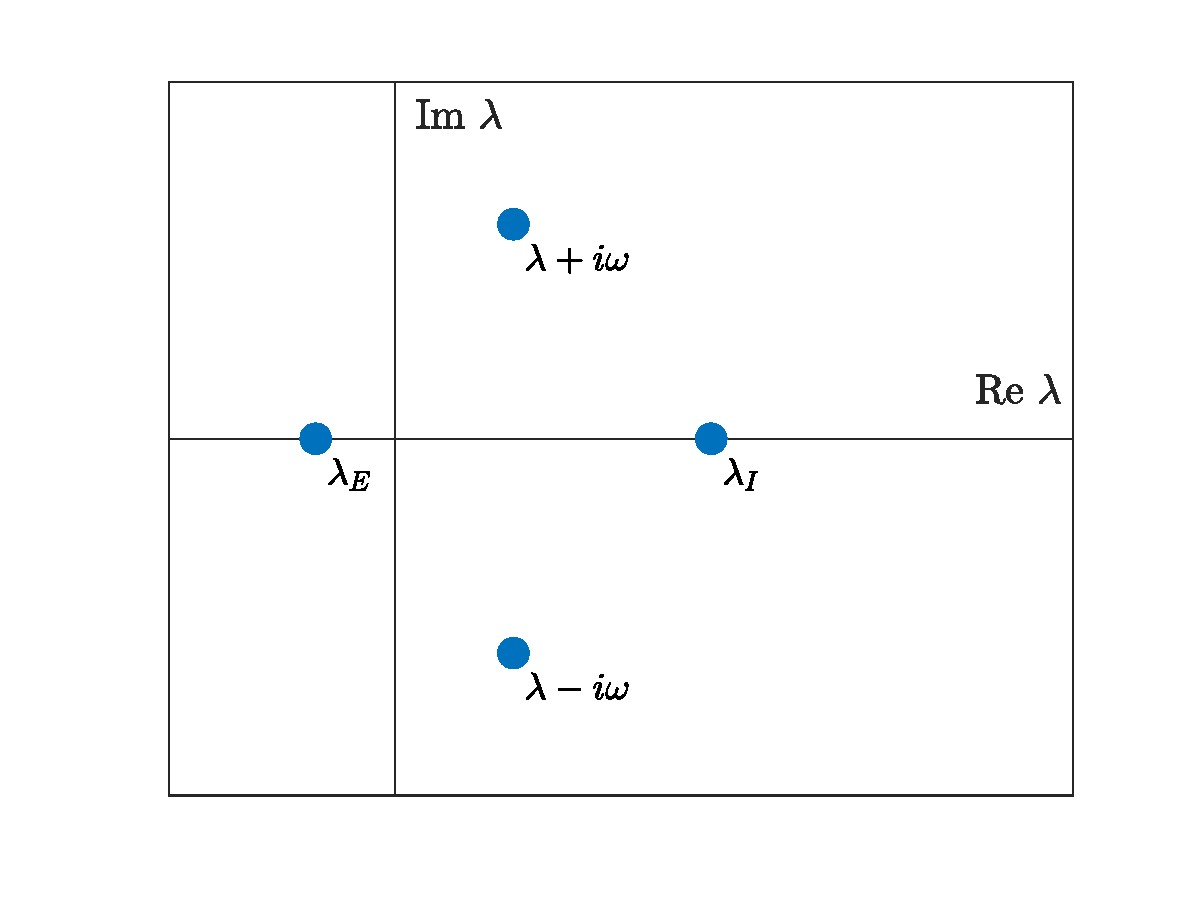
\includegraphics[width=7cm]{images/eigpattern1.eps} &
    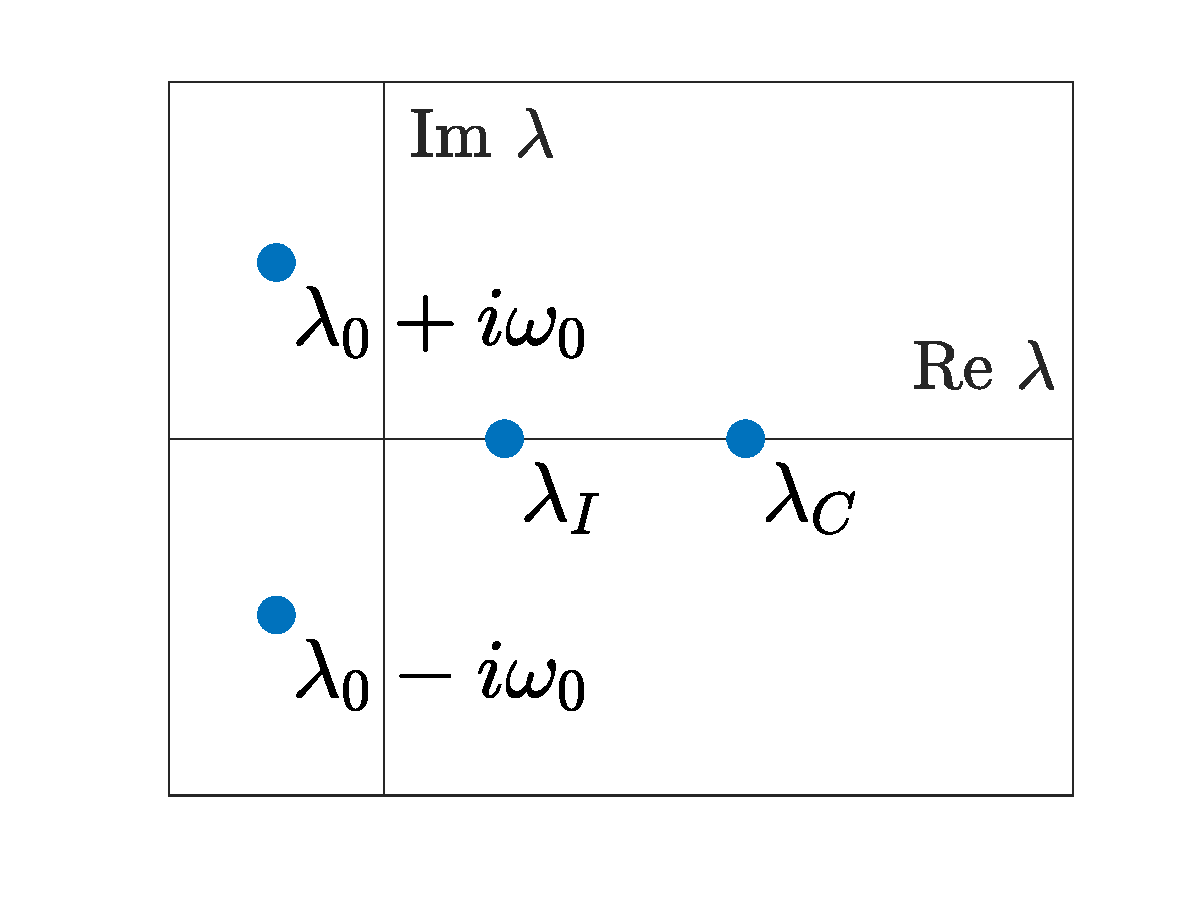
\includegraphics[width=7cm]{images/eigpattern2.eps} \\
    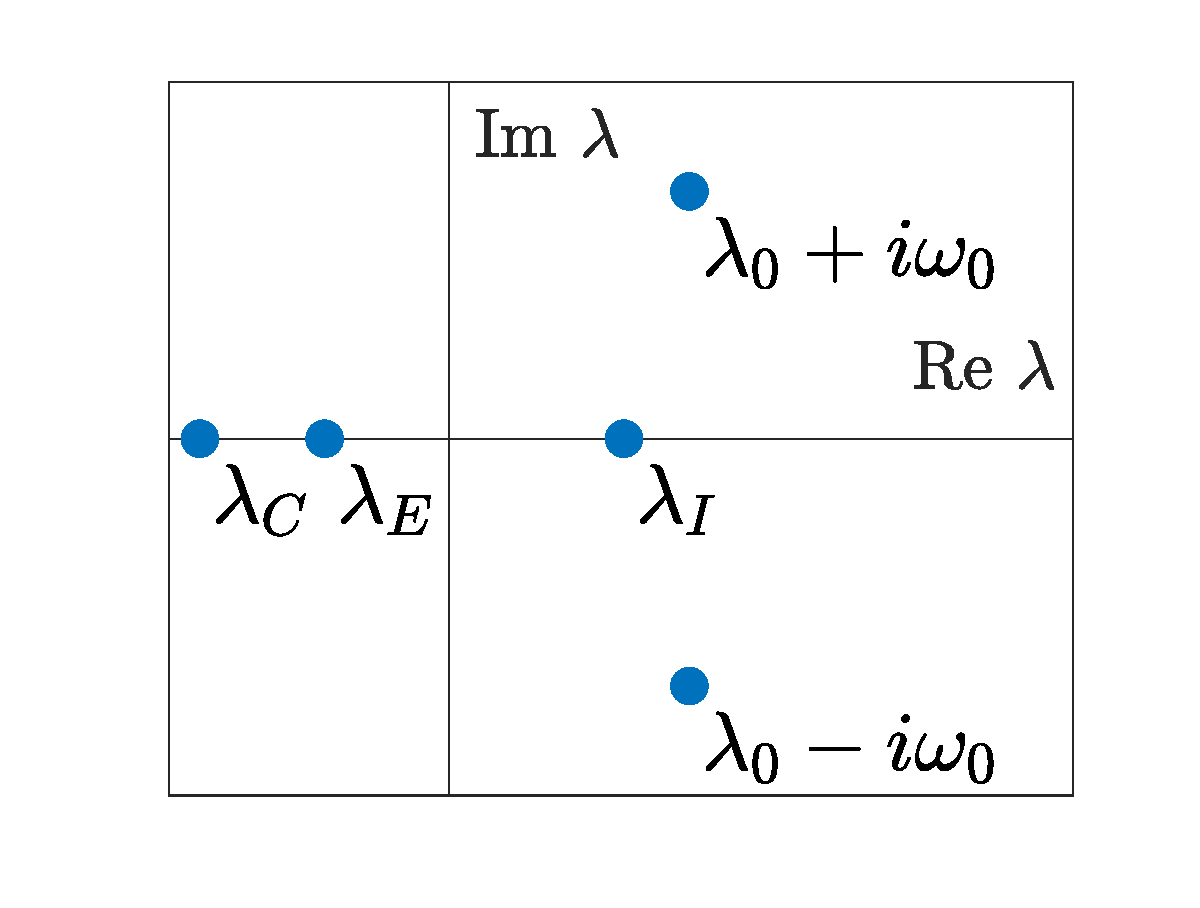
\includegraphics[width=7cm]{images/eigpattern3.eps} &
    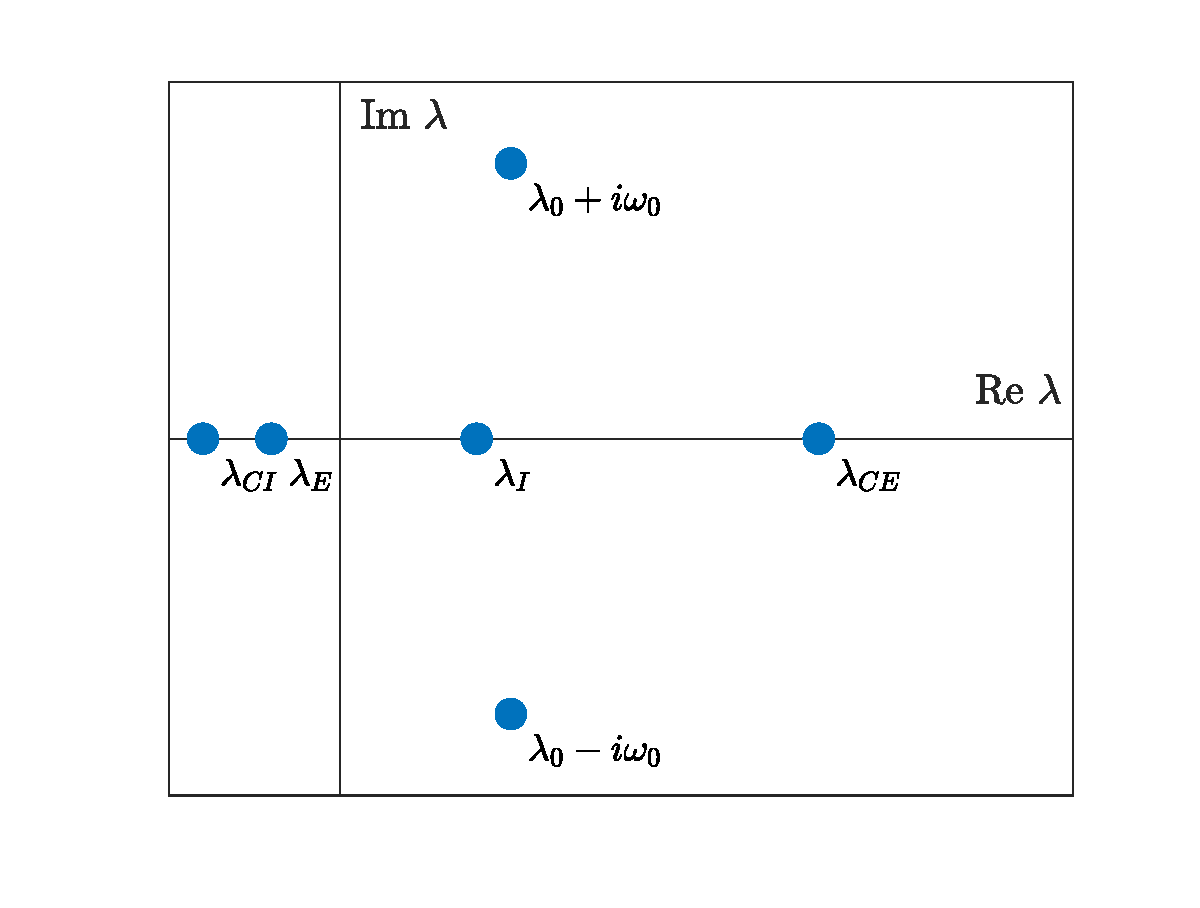
\includegraphics[width=7cm]{images/eigpattern4.eps} 
    \end{tabular}
    \caption{Eigenvalue pattern of connectivity matrix $H$ for single excitatory and single inhibitory cluster (top left), multiple excitatory clusters and single inhibitory cluster (top right), single excitatory cluster and multiple inhibitory clusters (bottom left), and multiple excitatory and inhibitory clusters (bottom right). }
    \label{fig:Heigpattern}
\end{figure}

We first reported on this phenomenon in \cite{Barreiro2017}, where we analyzed all-to-all connected, balanced excitatory-inhibitory networks. In this paper, we first flesh out some details about that system (say more). We then extend the analysis to several families of networks, which share...

For the remainder of this paper we will use $f = 0.8$ for a 4-to-1 excitatory-to-inhibitory ratio, which is typical for cortical networks [REFERENCE].

\section{Model simplification}

Since we are interested in locating fixed points and periodic orbits, we can simplify the model by using the fact that all excitatory cells within each cluster must be synchronized at a fixed point or periodic orbit. In the case where there is a single excitatory cluster, if $x_1$ and $x_2$ are the activities of two excitatory cells, then it follows from \cite{Barreiro2017} that
\begin{align}\label{eq:dt_x1t2diff}
\frac{d}{dt}|x_1 - x_2|^2 \leq -2 |x_1 - x_2 |^2.
\end{align}
The only way this can be true for a fixed point (for which $\frac{d}{dt} |x_1 - x_2|^2 =0$) or for a periodic orbit (for which $x_1(t)-x_2(t) = x_1(t+T)-x_2(t+T)$ for some period $T$) is if $x_1(t) = x_2(t)$ for all $t$. If $x_1$ and $x_2$ are the activities of two cells in the same excitatory cluster, equation \cref{eq:dt_x1t2diff} holds by the same argument as in \cite{Barreiro2017}, since both neurons receive the same incoming connections with the same weights. 

For the case where there is a single cluster of inhibitory cells ($n_{CI} = 1$), if there are $n_C$ excitatory clusters containing $p$ cells each, and $n_I$ inhibitory cells ($N = pN_c + N_i$ total cells), equation \cref{eqn:sys_Basic} then reduces to the system of $n_C + n_I$ equations
\begin{equation}\label{eq:reducedsystem}
\begin{aligned}
\dot{x}_{Ej} &= -x_{Ej} + \frac{(p-1)}{\sqrt{N}}\mu_{EE} \tanh(g x_{Ej}) + \frac{1}{\sqrt{N}} \mu_{EI} \sum_k \tanh(g x_{Ik}) && j = 1, \dots, n_C \\
\dot{x}_{Ij} &= -x_{Ij} + \frac{p}{\sqrt{N}}\mu_{IE} \sum_k \tanh(g x_{Ek}) + \frac{1}{\sqrt{N}} \mu_{II} \sum_{k\neq j}  \tanh(g x_{Ik}) && j = 1, \dots, n_I
\end{aligned}
\end{equation}
$x_{Ej}$ is the activity for the excitatory cluster $j$, and $x_{Ij}$ is activity for the inhibitory cell $j$. In matrix form, equations \cref{eq:reducedsystem} can be written
\begin{equation}\label{eq:reducedmatrixform}
\dot{\xvec} = \tilde{F}(\xvec, g) := -\xvec + \frac{1}{\sqrt{N}} \tilde{H} \tanh(g \xvec),
\end{equation}
where $\xvec = (x_{E_1}, \dots, x_{E_{n_C}}, x_{I_1}, \dots, x_{I_{n_I}})^T$, and $\tilde{H}$ is the $(n_C + n_I) \times (n_C + n_I)$ matrix
\[
\tilde{H} = \left[ \begin{array}{c|c}
    \\
    (p-1) \mu_{EE} I_{n_C} & \mu_{EI} \Onevec_{n_C \times n_I}\\
    \\
    \hline
    \\
    p \mu_{IE} \Onevec_{n_I \times n_C} & \mu_{II} \mathbf{K}_{n_I} \\
    \\
    \end{array}
    \right]
\]
Let $\xvec^* = (x_{E_1}^*, \dots, x_{E_{n_C}}^*, x_{I_1}^*, \dots, x_{I_{n_I}}^*)^T$ be a fixed point of \cref{eq:reducedmatrixform}. The linearization of \cref{eq:reducedmatrixform} about $\xvec^*$ is the matrix
\begin{equation}\label{eq:DtildeFxstar}
    D\tilde{F}(\xvec^*) = \frac{g}{\sqrt{N}}\tilde{H}(\xvec^*) - I_{n_C+n_I}
\end{equation}
where 
\begin{equation}\label{eq:tildeHxstar}
\tilde{H}(\xvec^*) := \tilde{H} \text{diag}(\sech^2(g \xvec^* ))
\end{equation}
There is a corresponding fixed point $\xvec_0^*$ to \cref{eqn:sys_Basic}, where each $x_{E_j}^*$ in $\xvec^*$ is repeated $p$ times. Let $\vvec = (v_{E_1}, \dots, x_{E_{n_C}}, x_{I_1}, \dots, x_{I_{n_I}})^T$ be an eigenvector of $\tilde{H}(\xvec^*)$ with eigenvalue $\lambda$. By comparing $\tilde{H}(\xvec^*)$ and $H(\xvec_0^*)$, there is a corresponding eigenvector $\vvec_0$ to $H(\xvec_0^*)$ with eigenvalue $\lambda$, where $\vvec_0$ is obtained from $\vvec$ by repeating each entry $v_{E_j}$ $p$ times. The matrix $H(\xvec_0^*)$ has $n_E - n_C = (p-1)n_C$ eigenvalues which are not eigenvalues of $\tilde{H}(\xvec^*)$. For each $j=1,\dots,n_C$, it is straightforward to show that $H(\xvec_0^*)$ has an eigenvalue at $\lambda = -\sech^2(x_{E_j}) \mu_{EE}$ with multiplicity $p-1$. (For $j=1$, for example, the $p-1$ eigenvectors are $\vvec^1, \dots, \vvec^{p-1}$, where $v^k_1 = -1$, $v^k_{k+1} = 1$, and all other components are 0). Since $\mu_{EE} > 0$, these eigenvalues are always negative. The corresponding eigenvalues of $DF(\xvec_0^*)$ will be negative for all $g$ and will have no effect on the stability of $x_0^*$. It therefore suffices to use the reduced system to determine stability of fixed points.
 
\section{Single excitatory and inhibitory cluster}\label{sec:E1I1}

The simplest case (considered in \cite{Barreiro2017}) involves a single excitatory cluster and a single inhibitory cluster. The matrix $H$ reduces to
\[
H = 
\left[ \begin{array}{c|c}
\\
\mu_{EE} \Kvec_{n_E} & \mu_{EI} \Onevec_{n_E \times n_I}\\
\\
\hline
\\
\mu_{IE} \Onevec_{n_I \times n_E} & \mu_{II} \mathbf{K}_{n_I} \\
\\
\end{array}
\right]
\]
We choose the weights so that the network is \emph{balanced}; that is, the excitatory and inhibitory currents coming into each cell should approximately cancel (CITE Rajan and Abbott). To achieve this balance, we set $\mu_{EI} = -\alpha \mu_{EE}$ and $\mu_{II} = -\alpha \mu_{IE}$, where $\alpha = \frac{f}{1-f}$. For simplicity, we also take $\mu_{IE} = \mu_{EE}$. The spectrum of $H$ is now easy to compute \cite{Barreiro2017}. The eigenvalues of $H$ (top left panel of \cref{fig:Heigpattern}) are
\begin{itemize}
    \item $\lambda_I := \alpha \mu_{EE} > 0$ with multiplicity $n_I - 1$
    \item $\lambda_E := -\mu_{EE} < 0$ with multiplicity $n_E - 1$
    \item One complex pair $\lambda_0 \pm i \omega_0$, with $\lambda_0 := \mu_{EE}\frac{\alpha - 1}{2}$ and $\omega_0 := \mu_{EE}\sqrt{\alpha+1}\sqrt{n_E - \frac{\alpha+1}{4}}$. 
\end{itemize}
It is straightforward to check that $\lambda_E < 0 < \lambda_0 < \lambda_I$. As discussed above, all bifurcations of $\xvec = 0$ involve only $\lambda_0 \pm i \omega_0$ and $\lambda_I$, which are the eigenvalues of $H$ with positive real part.

\subsection{Bifurcations of the origin}

As the bifurcation parameter $g$ is increased from 0, the eigenvalues of $DF(0)$ corresponding to $\lambda_I$ crosses the imaginary axis at
\begin{equation}\label{eq:pitchlocation}
    g = g_0 := \frac{\sqrt{N}}{\alpha \mu_{EE}}.
\end{equation}
As $g$ is further increased, the complex pair of eigenvalues of $DF(0)$ crosses the imaginary axis at 
\begin{equation}\label{eq:0hopflocation}
    g= g_H := \frac{ 2\sqrt{N} }{ (\alpha-1)\mu_{EE} }.
\end{equation}
The origin $\xvec = 0$ is a stable equilibrium for $g < g_0$, at which point it loses stability in a symmetric pitchfork bifurcation, where $n_I -1$ eigenvalues cross the imaginary axis simultaneously. 

At $g = g_H$, the origin undergoes a Hopf bifurcation. The frequency of the limit cycle which emerges at the Hopf bifurcation is given by the imaginary part of the complex pair of eigenvalues at $g = g_H$, which is $\omega_H(N) = \frac{2}{\alpha-1}\sqrt{\alpha+1}\sqrt{f N- \frac{\alpha+1}{4}} -1$, where we used $n_E = f N$. In particular, we note that $\omega_H(N) \rightarrow \infty$ as $N \rightarrow \infty$.

For $g > g_H$, numerical computation shows that there is a limit cycle for which all excitatory cells are synchronized and all inhibitory cells are synchronized. We can argue that such a limit cycle exists for $g > g_H$ by reducing \cref{eqn:sys_Basic} to the two-dimensional system
\begin{equation}\label{eq:2dsystem}
\begin{aligned}
\dot{x} &= f(x, y) := -x + \frac{\mu_{EE}}{\sqrt{N}}\left((n_E - 1) \tanh(g x) - \alpha n_I \tanh(g y) \right) \\
\dot{y} &= g(x, y) := -y + \frac{\mu_{EE}}{\sqrt{N}}\left( n_E \tanh(g x) - \alpha (n_I - 1) \tanh(g y) \right), 
\end{aligned}
\end{equation}
where $x$ represents the synchronized excitatory cell activity and $y$ represents the synchronized inhibitory cell activity. $(x, y) = (0, 0)$ is always a fixed point of \cref{eq:2dsystem}. Since $-1 < \tanh x < 1$, we can solve $f(x, y) = 0$ for $y$ in terms of $x$ when $|x| < \frac{\mu_{EE}}{\sqrt{N}}( 2 \alpha n_I - 1)$ to get the equation for the $x$-nullcline.
\begin{align*}
y = \frac{1}{g} \tanh ^{-1} \left( \tanh (g x) - \frac{ \mu_{EE} \tanh (g x) + \sqrt{N} x}{\alpha \mu_{EE} n_I} \right).
\end{align*}
Similarly we can solve $g(x, y) = 0$ for $x$ in terms of $y$ when $|y| < \frac{\alpha \mu_{EE}}{\sqrt{N}}$ to get the equation for the $y$-nullcline. The two nullclines are plotted in the left panel of \cref{fig:nullclines}. We will assume that the nullclines intersect only at the origin as in \cref{fig:nullclines}. This implies that $(x,y) = (0,0)$ is the only equlibrium point of \cref{eq:2dsystem}. 

Linearizing about the origin \cref{eq:2dsystem} yields the $2 \times 2$ matrix
\[
\frac{g \mu_{EE}}{\sqrt{N}}
\begin{bmatrix} 
n_E - 1 & -\alpha n_I \\
n_E & -\alpha(n_I - 1)
\end{bmatrix} - I_2
\]
which has a complex conjugate pair of eigenvalues $\frac{g}{\sqrt{N}}(\lambda_0 \pm \omega_0) - 1$, where $\lambda_0$ and $\omega_0$ are defined above. Thus the origin is unstable for $g > g_H$, which is the Hopf bifurcation point defined by \cref{eq:0hopflocation}. To show there is a limit cycle for $g > g_H$, we use the Poincare-Bendixson theorem. We draw a square around the origin with corners $(-a, -a)$ and $(a, a)$. On the line $x = a$, for $a$ large, 
\[
\dot{x} \leq -a + \frac{2 n_E}{\sqrt{N}} = -a + 2 f \sqrt{N},
\]
which can be made negative by taking $a$ sufficiently large. Similarly, we can take $a$ sufficiently large so that the vector field defined by Fig. \ref{eq:2dsystem} points inward at all points on the square (see right panel of \cref{fig:nullclines}). Since the origin is repelling for $g > g_H$, it follows from the Poincare-Bendixson theorem that there is a limit cycle surrounding the origin for $g > g_H$. Although we note that this limit cycle is stable for the system \cref{eq:2dsystem}, the theorem says nothing about its stability in the larger system \cref{eq:reducedsystem}.

\begin{figure}
    \centering
    \begin{tabular}{cc}
    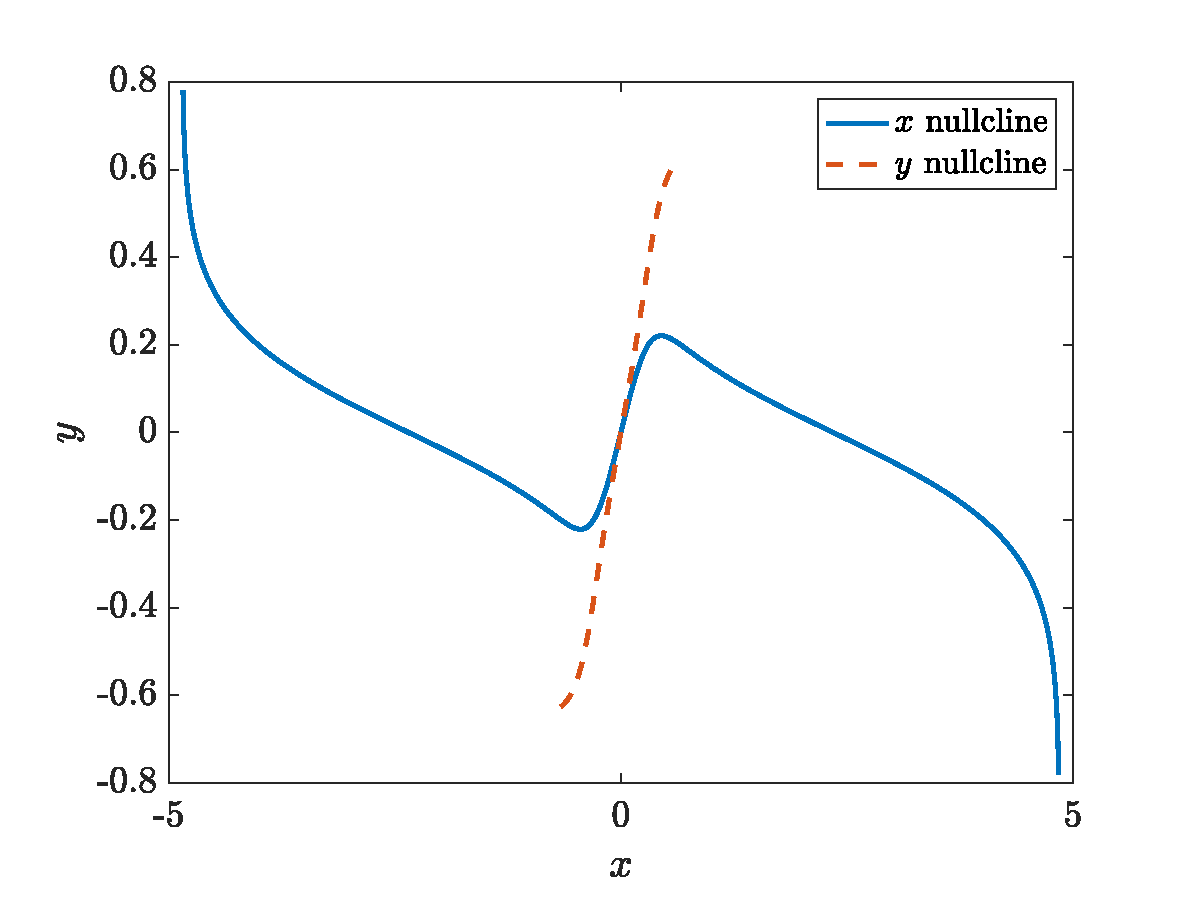
\includegraphics[width=8cm]{images/nullclines.eps} &
    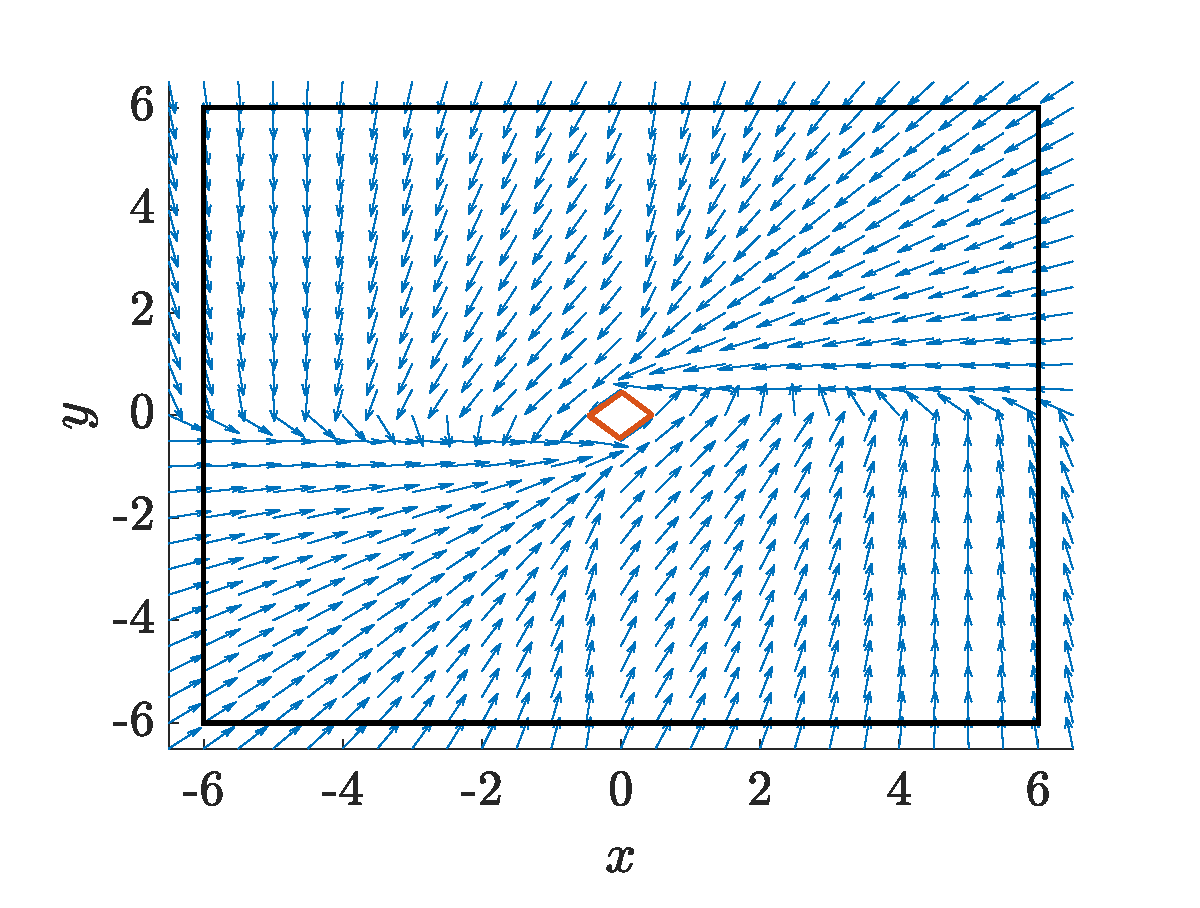
\includegraphics[width=8cm]{images/trappingregion.eps}
    \end{tabular}
    \caption{Left panel shows $x$ and $y$ nullclines for the system \cref{eq:2dsystem}. Right panel shows the slope fields for \cref{eq:2dsystem}, with a small limit cycle visible in center.  Slope field points inward on black box. $N = 20$, $g = 5$, $\alpha = 4$, and $\mu_{EE} = 0.7$.}
    \label{fig:nullclines}
\end{figure}


\subsection{Solutions after symmetric pitchfork bifurcation}
These solutions merit some discussion, because this is where symmetry comes into play.  Our main tool is the \emph{Equivariant Branching Lemma}, which tells us what type of solutions to \cref{eqn:sys_Basic} will arise at bifurcation points, when symmetries are present \cites{MR631456,GSS88Vol2,HoyleRebeccaB2006Pf:a}. Before stating this result, we introduce some terminology. Let $\Gamma$ be a finite group acting on $\mathbb{R}^N$; then we say that a mapping $F: \mathbb{R}^N  \rightarrow \mathbb{R}^N$ is \textit{$\Gamma$-equivariant} if $F(\gamma \xvec) = \gamma F(\xvec)$, for all $\xvec \in \mathbb{R}^N$ and $\gamma \in \Gamma$.  A one-parameter family of mappings $F: \mathbb{R}^N \times \mathbb{R}  \rightarrow \mathbb{R}^N$ is \textit{$\Gamma$-equivariant}, if it is $\Gamma$-equivariant for each value of its second argument.

We say that $V$, a subspace of $\mathbb{R}^N$,  is \textit{$\Gamma$-invariant} if $\gamma \vvec \in V$, for any $\vvec$ and $\gamma \in \Gamma$. We furthermore say that the action of $\Gamma$ on $V$ is \textit{irreducible} if $V$ has no proper invariant subspaces; i.e. the only $\Gamma$-invariant subspaces of $V$ are $\{0\}$ and $V$ itself. 

For a group $\Gamma$ and a vector space $V$, we define the \textit{fixed-point subspace} for $\Gamma$, denoted $\rm{Fix} (\Gamma)$, to be all points in $V$ that are unchanged under any of the members of $\Gamma$; i.e. $\rm{Fix} (\Gamma) = \{ \xvec \in V : \gamma \xvec = \xvec, \forall \gamma \in \Gamma \}$. 
%\Acomment{Note that isotropy subgroup has two meanings: check that I am correct about this} 
The \textit{isotropy subgroup of $\xvec \in V$}, denoted $\Sigma_x$, is the set of all members of $\Gamma$ under which $\xvec$ is fixed; i.e. $\Sigma_x = \{ \gamma \in \Gamma : \gamma \xvec = \xvec \}$ (we then say that a subgroup $\Sigma$ is \textit{an} isotropy subgroup of $\Gamma$, if it is the isotropy subgroup, $\Sigma_x$, for some $\xvec \in V$.)\\

Suppose we have a one-parameter family of mappings, $F(\xvec, g)$, and we wish to solve $F(\xvec, g)=0$. 
For any $(\xvec, g) \in \mathbb{R}^n \times \mathbb{R}$, let $(dF)_{\xvec,g}$ denote the $N \times N$ Jacobian matrix 
\[ \left( \frac{\partial F_j}{\partial x_k} (\xvec, g) \right)_{j, k=1...N}
\] 
A bifurcation will occur when the Jacobian ceases to be invertible --- when $(dF)_{\xvec,g}$ has a nontrivial kernel. For a $\Gamma$-equivariant mapping --- i.e. $F(\xvec,g)$ is $\Gamma$-equivariant for any value of the parameter $g$ --- we may have \textit{multiple} eigenvalues go through zero at once, because of symmetries; however, the structural changes that occur are qualitatively the same as those that occur in a non-symmetric system, with a single zero eigenvalue. 
Furthermore, we will have \textit{multiple} such solution branches, each corresponding to a subgroup of the original symmetries.  The following Lemma formalizes this fact:

%Then the Implicit Function Theorem states that we can continue to track a unique solution branch as a function of $g$, as long as the Jacobian remains invertible. When this ceases to be true --- when $(dF)_{\xvec,g}$ has a nontrivial kernel --- we have the possibility for a bifurcation. At this point the number of zero eigenvalues (whether there are one, or two, etc..) and a menagerie of further conditions will determine the qualitative properties of the structural change that occurs.
%that is $\rm{det} dF \not= 0$, where $dF_{jk} = \left( \frac{\partial F_j}{\partial x_k} \right)  It states conditions for 

%What complicates this situation for $\Gamma$-equivariant mappings --- i.e. $F(\xvec,g)$ is $\Gamma$-equivariant for any value of the parameter $g$ --- is that because of symmetries, \textit{multiple} eigenvalues will go through zero at once; however, the structural changes that occur are qualitatively the same as those that occur in a non-symmetric system, with a single zero eigenvalue. What changes is that we now have \textit{multiple} such solution branches, each corresponding to a subgroup of the original symmetries.  The following Lemma formalizes this fact:\\


\begin{thm} (Equivariant Branching Lemma: paraphrased from \cite{GSS88Vol2}, pg. 82, see also pg. 67-69 ): Let $F: \mathbb{R}^N \times \mathbb{R} \rightarrow \mathbb{R}^N$ be a one-parameter family of $\Gamma$-equivariant mappings with $F(\xvec_0, g_0) = \Zerovec$. Suppose that $(\xvec_0, g_0)$ is a bifurcation point and that, defining $V = \ker(dF)_{\xvec_0, g_0}$, $\Gamma$ acts absolutely irreducibly on $V$. Let $\Sigma$ be an isotropy subgroup of $\Gamma$ satisfying 
\begin{eqnarray}
\rm{dim}\; \rm{Fix} (\Sigma) = 1,
\end{eqnarray}
where $\rm{Fix (\Sigma)}$ is the \emph{fixed-point subspace} of $\Sigma$: that is, $\rm{Fix} (\Sigma) \equiv \{ x \in V \mid \sigma x = x, \;  \forall \sigma \in \Sigma \}$. Then there exists a unique smooth solution branch to $F = 0$ such that the isotropy subgroup of each solution is $\Sigma$. \\
\end{thm}

The reader can readily check that the right-hand side of Eqn. \eqref{eqn:sys_Basic} is $\Gamma$-equivariant, for $\Gamma = S_{n_E} \times S_{n_I}$, where $S_n$ is the group of permutations on $n$ objects. That is, we can permute the labels on the excitatory cells, and/or the labels on the inhibitory cells, without changing the equations.

At $g=g_0$, $n_I -1$ eigenvalues pass through zero: the corresponding eigenspace is the set of all zero-sum vectors with support in the inhibitory cells only; i.e. 
\[ V \equiv  \ker(dF)_{\Zerovec,g^{\ast}}  = {\rm span} \, \{ \left[  
\underbrace{\begin{matrix}0 & \cdots & 0\end{matrix}}_{n_{E}} \;
\vvec_{n_{I}} \right] \}, \qquad \vvec_{n_{I}} \perp \Onevec_{n_{I}}.\]
To check that $\Gamma$ acts irreducibly on $V$ it is sufficient to show that the subspace spanned by the \textit{orbit} of a single vector $\vvec$ (defined as the set of all values  $\gamma \vvec$, for $\gamma \in \Gamma$) is full rank; this can be readily confirmed for $\vvec_{n_{I}} = \left[ \begin{array}{ccccc} 1 & -1 & 0 & ... & 0 \end{array} \right]$, for example.   

To find the appropriate subgroup of symmetries, break the inhibitory cells up into precisely two clusters and retain only permutations within each cluster. This describes a subgroup of $\Gamma$, $\Sigma = S_{n_E} \times S_{n_{I_1}} \times S_{n_{I_2}}$, $n_{I_1} + n_{I_2} = n_I$.
Assuming that (without loss of generality) the $I_1$ neurons have the indices $n_E+1,...,n_E+n_{I_1}$, and so forth, $\Sigma$ has the fixed point subspace 
\begin{eqnarray}
\rm{Fix}(\Sigma) & = & {\rm span} \, \{ \left[  
\underbrace{\begin{matrix}0 & \cdots & 0\end{matrix}}_{n_E} \;
\underbrace{\begin{matrix}1 & \cdots & 1\end{matrix}}_{n_{I_1}} \;
\underbrace{\begin{matrix}-\frac{n_{I_1}}{n_{I_2}} & \cdots & -\frac{n_{I_1}}{n_{I_2}} \end{matrix}}_{n_{I_2}} \right] \}
\end{eqnarray}
We can check that $\rm{Fix}(\Sigma)$ is a subspace of $V$; furthermore $\dim \rm{Fix}(\Sigma) = 1$ because it can be described as the span of a single vector. 

As a consequence, there is a branch of solutions emerging at the bifurcation point $g=g_0$ for any possible division of the inhibitory cells into exactly two clusters. We refer to these as $I_1/I_2$ branches.  Each such branch may be characterized by the number $\beta = n_{I_1}/n_{I_2}$, which gives the ratio of the cluster sizes. Without loss of generality, we may take $n_{I_1} \geq n_{I_2}$, so that $\beta \geq 1$. Each cluster of inhibitory cells is synchronized.

\subsection{Solutions along $I_1/I_2$ branches}

The simplest case occurs when $n_I$ is even and $\beta = 1$, in which case $n_{I_1}=n_{I_2}$. On this branch, $x_E = 0$, and $x_{I_2} = -x_{I_1}$, i.e. there are two equally sized inhibitory populations with equal and opposite activities. Letting $x_{I_1} = x_I$, substituting these into \cref{eq:otherbranchmatrixeq}, and simplifying, we obtain the single equation (\cite{Barreiro2017}*{Eq. 16})
\[
-x_I + \frac{\alpha \mu_{EE} }{\sqrt{N}} \tanh(g x_I) = 0, 
\]
which simplifies to 
\begin{equation}\label{eq:xIbrancheq}
\tanh(g x_I) = g_0 x_I
\end{equation}
Expanding the LHS of \cref{eq:xIbrancheq} in Taylor series about $g x_I = 0$,
\begin{equation}\label{eq:tanhTaylor}
g x_I - \frac{(g x_I)^3}{3} + \frac{2(g x_I)^5}{15} + \mathcal{O}\left( (g x_I)^7 \right) = g_0 x_I
\end{equation}
Keeping up to cubic terms, equation \cref{eq:tanhTaylor} simplifies to
\[
x_I \left( (g - g_0) - \frac{g^3}{3} x_I^2 \right) = 0,
\]
thus for $g$ close to $g_0$, the nonzero solution for $x_I$ is given, to leading order, by
\begin{align}\label{eq:xIapprox}
x_I &= \sqrt{ \frac{3(g - g_0) }{g^3}} && g \geq g_0.
\end{align}
We can obtain a higher-order approximation by keeping up to fifth-order terms in \cref{eq:tanhTaylor} to get
\begin{equation*}
x_I \left( (g - g_0) - \frac{g^3}{3} x_I^2 + \frac{2 g^5}{15} x_I^4 \right) = 0,
\end{equation*}
which is $x_I$ multiplied by a quadratic in $x_I^2$. To find the nonzero solution for $x_I$, we solve this quadratic for $x_I^2$ and take square roots to get, to leading order,
\begin{align}\label{eq:xIapprox5}
x_I &= \frac{1}{2} \sqrt{ \frac{5}{g^2} - \frac{\sqrt{ 5 g^5( 24 g_0 - 19 g) }}{g^5}} && g \geq g_0.
\end{align}
Comparison between the third-order approximation, the fifth-order approximation, and the numerical solution obtained by parameter continuation is shown in the left panel of \cref{fig:xIapprox}.

\begin{figure}
    \centering
    \begin{tabular}{cc}
    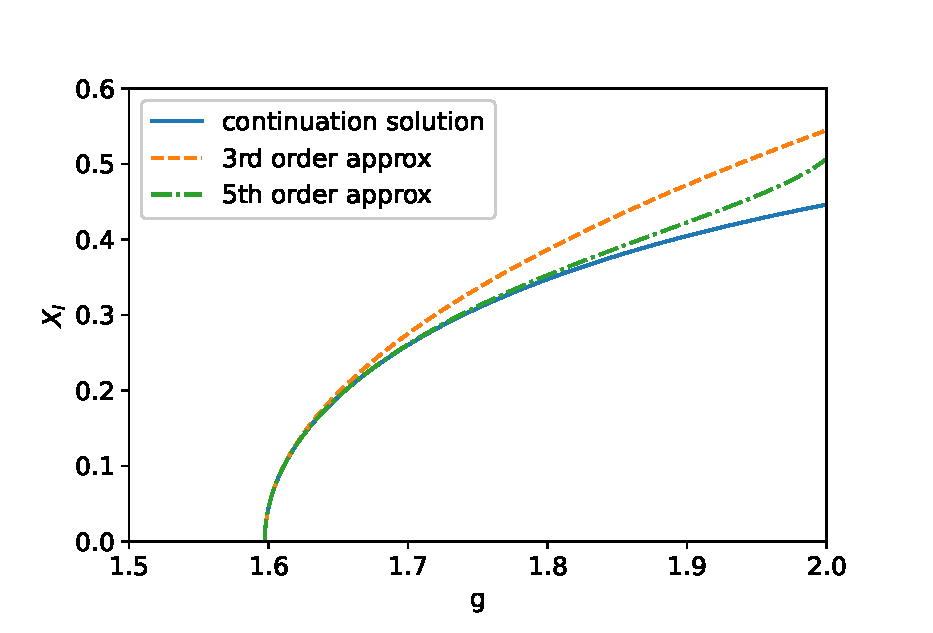
\includegraphics[width=8cm]{images/Xiapprox.eps} &
    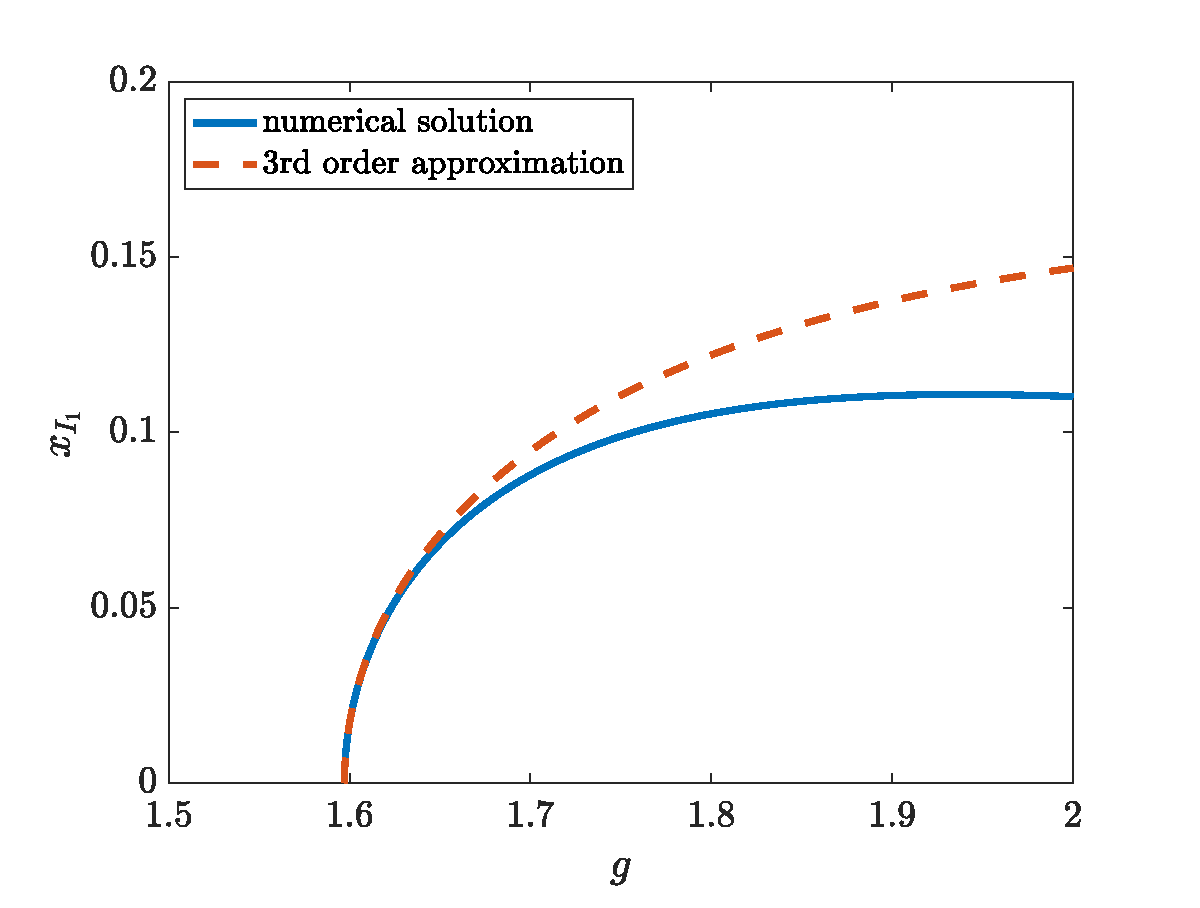
\includegraphics[width=8cm]{images/Xiapproxbeta3.eps} 
    \end{tabular}
    \caption{Third order approximation \cref    {eq:xIapprox} and fifth order approximation \cref{eq:xIapprox5} to $x_I$ on the $I_1=I_2$ branch of fixed points (left panel). Third order approximation \cref{eq:XI1} to $X_{I_1}$ on the $\beta=3$ branch (right panel). $N = 20$,  $\alpha = 4$, $\mu_{EE} = 0.7$.}
    \label{fig:xIapprox}
\end{figure}

For $\beta \neq 1$, we find the solution along each $I_1/I_2$ branch by reducing \cref{eqn:sys_Basic} to the 3-dimensional system
\begin{equation}\label{eq:otherbranchmatrixeq}
 \begin{aligned}
 \begin{bmatrix} x_E\\x_{I_1}\\x_{I_2}\end{bmatrix} 
 &= \frac{\mu_E}{\sqrt{N}} 
 \begin{bmatrix} (\alpha n_I - 1) & -\alpha \frac{\beta}{\beta+1} n_I & - \alpha \frac{1}{\beta+1} n_I  \\
    \alpha n_I  & -\alpha \left(\frac{\beta}{\beta+1} n_I-1\right) & - \alpha \frac{1}{\beta+1} n_I  \\
    \alpha n_I & -\alpha \frac{\beta}{\beta+1} n_I & -\alpha \left(\frac{1}{\beta+1} n_I-1\right)
 \end{bmatrix}
 \begin{bmatrix} \tanh(g x_E) \\\tanh ( g x_{I_1} ) \\\tanh(g x_{I_2})\end{bmatrix},
 \end{aligned}
 \end{equation}
 where $x_E$ is the activity of the excitatory cells (which are all synchronized), $x_{I_1}$ and $x_{I_2}$ are the activities of the two inhibitory clusters, and we used $n_E = \alpha n_I$. For any solution $(x_E, x_{I_1}, x_{I_2})^T$ to \cref{eq:otherbranchmatrixeq}, $\xvec = (x_E, \dots, x_E, x_{I_1}, \dots, , x_{I_1}, x_{I_2}, \dots, x_{I_2})^T$ is an equilibrium solution to \cref{eqn:sys_Basic}, where $x_E$, $x_{I_1}$, and $x_{I_2}$ are repeated $n_E$, $n_{I_1}$, and $n_{I_2}$ times, respectively. As $N \rightarrow \infty$, numerical continuation with AUTO suggests that \cref{eq:otherbranchmatrixeq} has a solution
\begin{equation}\label{eq:I1I2asymp}
    x_{I_2} = -\beta x_{I_1} + \mathcal{O}\left( \frac{1}{N^2} \right), \quad 
    x_{I_1} = \mathcal{O}\left( \frac{1}{N} \right), \quad
     x_E = \mathcal{O}\left( \frac{1}{N^2} \right)
\end{equation}
Subtracting the second and third equations in \cref{eq:otherbranchmatrixeq}, we get
\[
 x_{I_1} - x_{I_2} = \frac{\alpha}{\mu_{EE}\sqrt{N}}\left( \tanh(g x_{I_1}) - \tanh(g x_{I_2}) \right)
 \]
Substituting \cref{eq:I1I2asymp} into this as an ansatz, expanding the $\tanh$ terms in a Taylor series to cubic order, and simplifying, we obtain the formula for $x_{I_1}$ in terms of $g$, for $g$ close to $g_0$
 \begin{align}\label{eq:XI1}
 x_{I_1} &= \sqrt{ \frac{ 3(g - g_0) }{ (1 - \beta + \beta^2 )g^3}} + \mathcal{O}\left( \frac{1}{N^2}\right)&& g \geq g_0.
\end{align}
Note that this reduces to \cref{eq:xIapprox} when $\beta = 1$. Comparison between this approximation and the numerical solution obtained by parameter continuation is shown in the right panel of \cref{fig:xIapprox}.

\begin{figure}
    \centering
    \begin{tabular}{cc}
    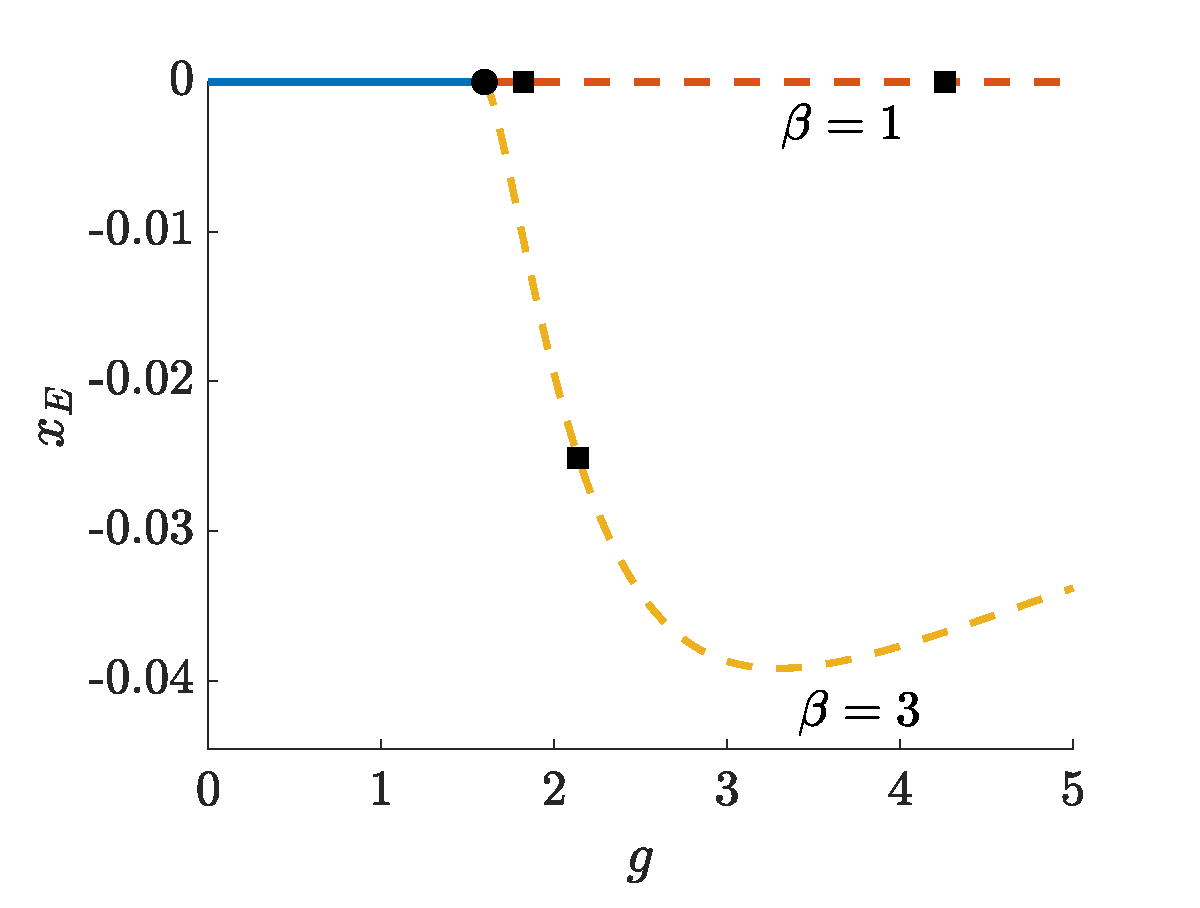
\includegraphics[width=8cm]{images/bdnoclusters20E.eps} &
    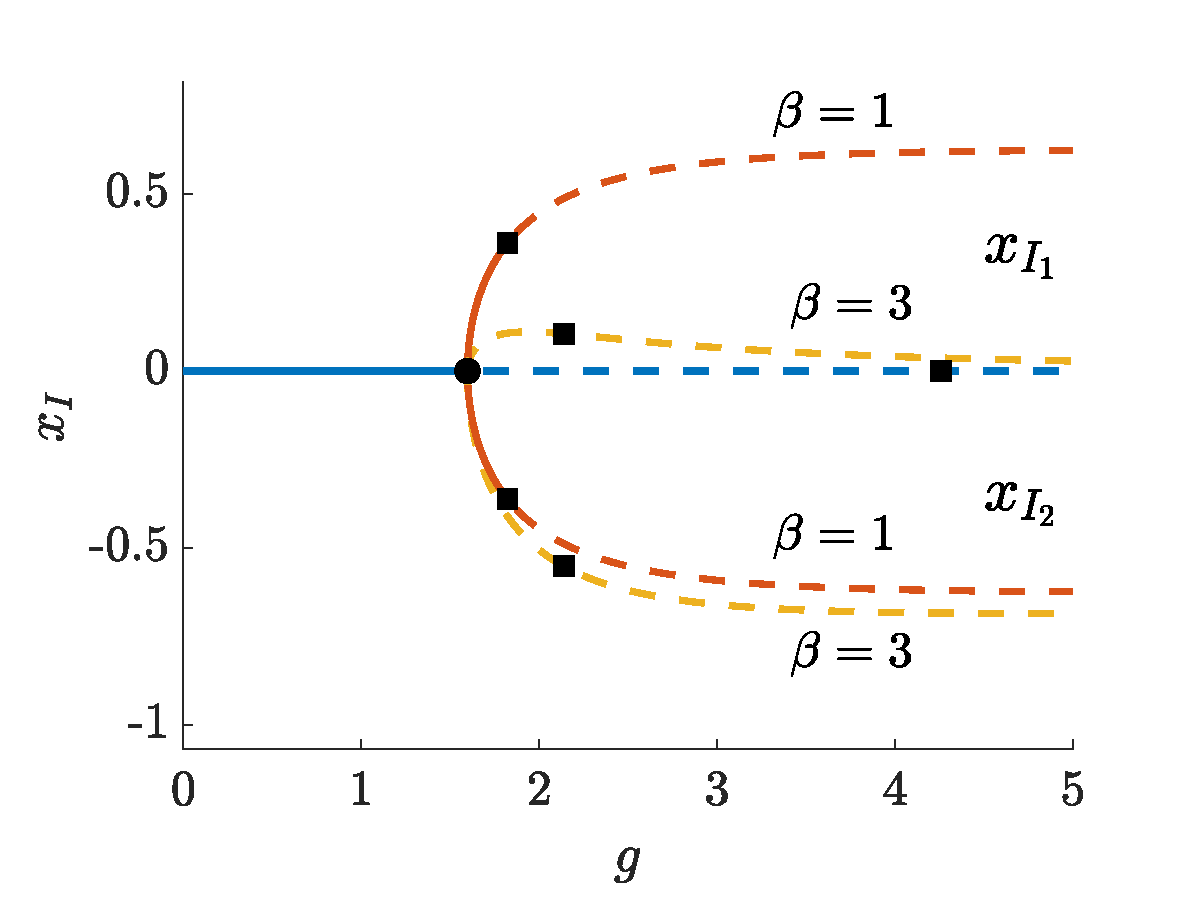
\includegraphics[width=8cm]{images/bdnoclusters20I.eps} \\
    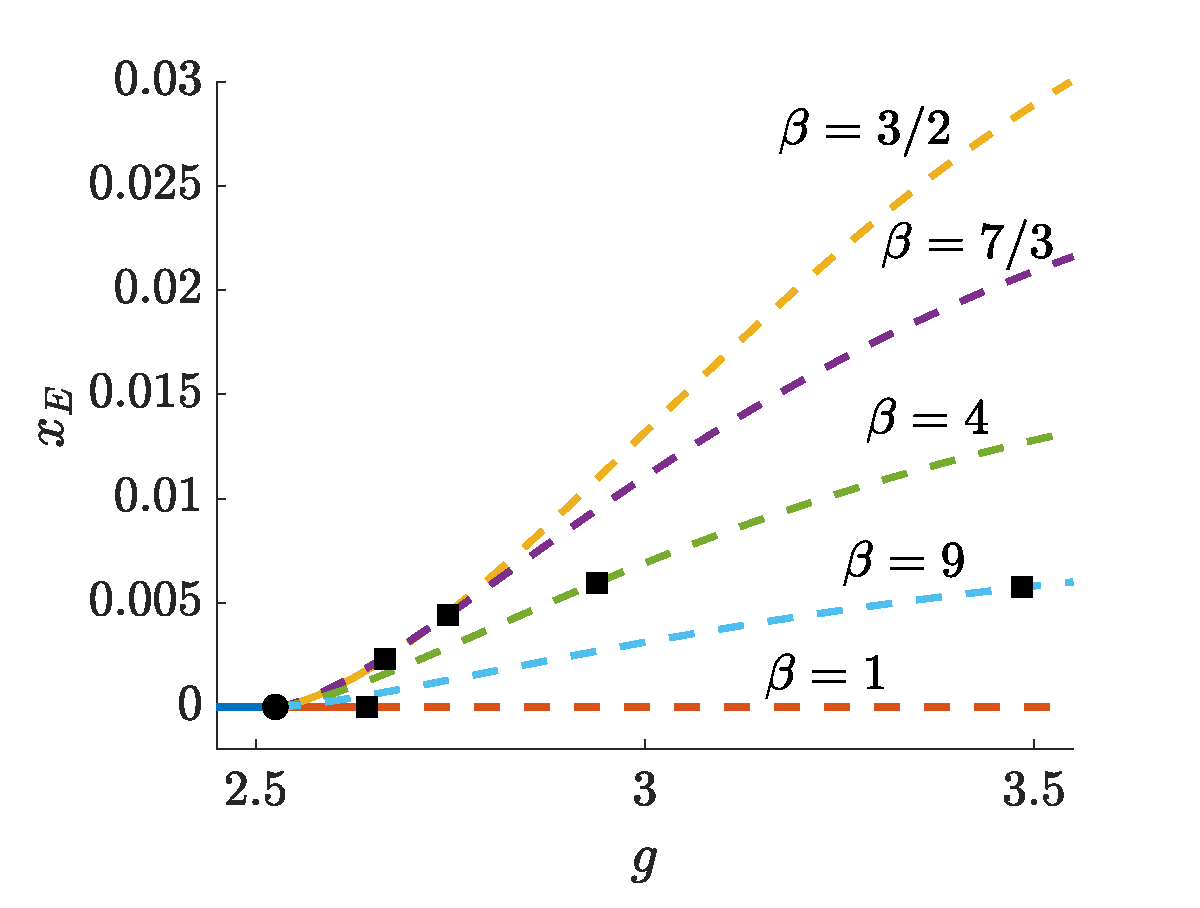
\includegraphics[width=8cm]{images/bdnoclusters50E.eps} &
    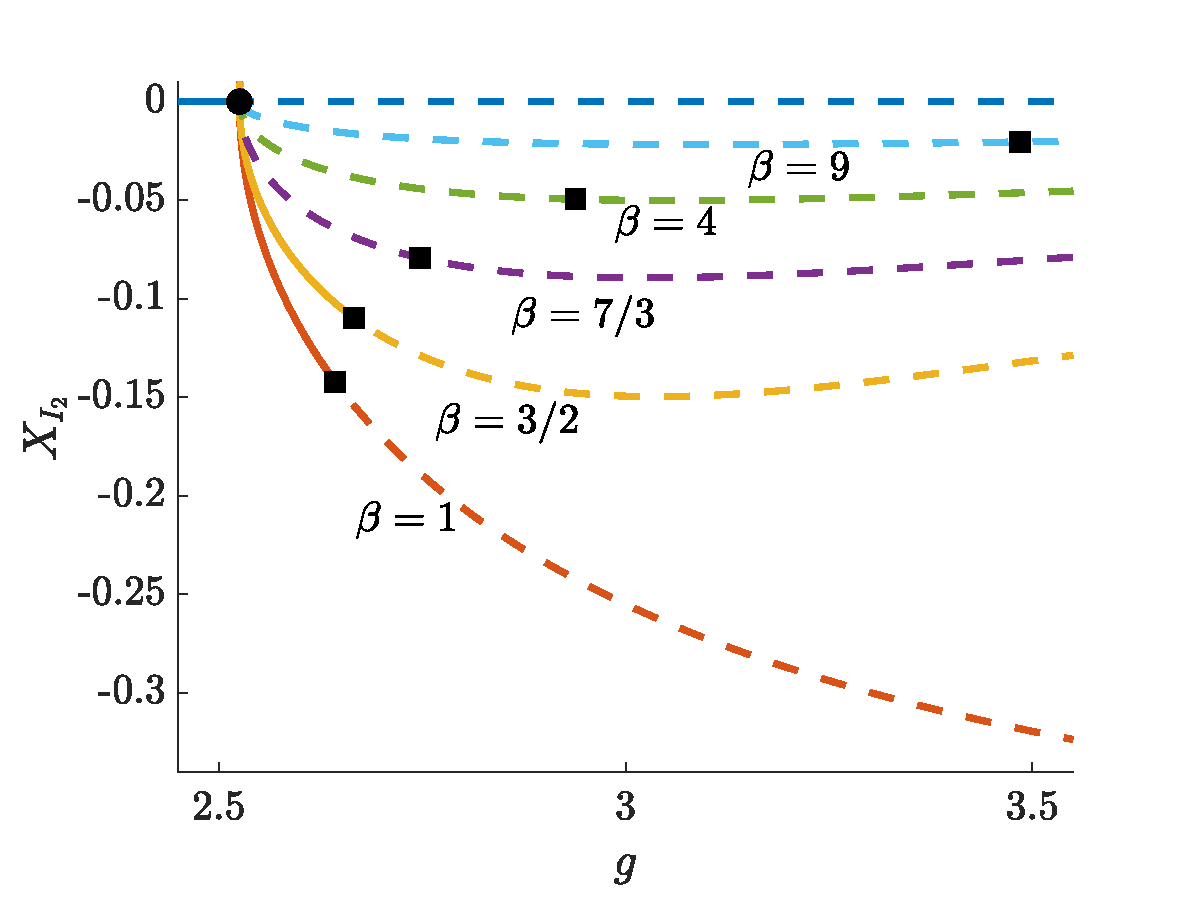
\includegraphics[width=8cm]{images/bdnoclusters50I.eps}
    \end{tabular}
    \caption{Bifurcation diagram showing $I_1/I_2$ branches of equlibria of \cref{eqn:sys_Basic} for all valid values of $\beta$. Top panels show $N=20$, with top left plotting $X_E$ vs $g$, and top right plotting $X_{I_1}$ (above horizontal axis) and $X_{I_2}$ (below horizontal axis) vs $g$. Bottom panels show $N=50$, with bottom left plotting $X_E$ vs $g$, and bottom right plotting $X_{I_2}$ only vs $g$. Solid lines indicate stable fixed points, dashed lines indicate unstable fixed points. Symmetric pitchfork bifurcation at $g = g_0$ indicated with filled circle. Hopf bifurcations indicated with filled squares. Further bifurcations along branches are not shown to avoid clutter. $\alpha = 4$, $\mu_{EE} = 0.7$.}
    \label{fig:noclusterBD1}
\end{figure}

\subsection{Stability and bifurcations along $I_1/I_2$ branches}

Choose any $\beta \geq 1$, so that $n_{I_1} = \frac{\beta}{\beta+1}n_I$ and $n_{I_2} = \frac{1}{\beta+1}n_I$, and let $\xvec = (x_E, x_{I_1}, x_{I_2})$ be a solution to \cref{eq:otherbranchmatrixeq} for $g > g_0$.To examine the stability and bifurcations which occur along the $I_1/I_2$ branches, we look at the linearization $D\tilde{F}(\xvec^*)$, where $\xvec^* = (x_E, x_{I_1}, \dots, x_{I_1}, x_{I_2}, \dots, x_{I_2})^T$, and $x_{I_1}$ and $x_{I_2}$ are repeated $n_{I_1}$ and $n_{I_2}$ times. As above, stability will depend on the eigenvalues of $\tilde{H}(\xvec^*)$. In doing this, we will also find a Hopf bifurcation along each $I_1/I/2$ branch, and can find an leading order formula for its location for large $N$.

First, we linearize the three-dimensional system \cref{eq:otherbranchmatrixeq} about the fixed point branch $(x_E, x_{I_1}, x_{I_2})$ to get the Jacobian
\[
J_3(\xvec) = \frac{g}{\sqrt{N}} H_3(\xvec) - I_3
\]
where 
\[
H_3(\xvec) = \mu_{EE}
 \begin{bmatrix} (\alpha n_I - 1) \sech^2(g x_E) & -\alpha \frac{\beta}{\beta+1} n_I \sech^2(g x_{I_1}) & - \alpha \frac{1}{\beta+1} n_I \sech^2(g x_{I_2}) \\
    \alpha n_I \sech^2(g x_E) & -\alpha \left(\frac{\beta}{\beta+1} n_I-1\right) \sech^2(g x_{I_1}) & -\alpha \frac{1}{\beta+1} n_I \sech^2(g x_{I_2}) \\
    \alpha n_I \sech^2(g x_E) & -\alpha \frac{\beta}{\beta+1} n_I \sech^2(g x_{I_1}) & -\alpha \left(\frac{1}{\beta+1} n_I-1 \right) \sech^2(g x_{I_2})
 \end{bmatrix}
\]
and $I_3$ is the $3 \times 3$ identity matrix. If $\lambda$ is an eigenvalue of $H_3(\xvec)$ with eigenvector $\vvec = (v_E, v_{I_1}, v_{I_2})$, then $\lambda$ is also an eigenvalue of $\tilde{H}(\xvec^*)$ with eigenvector $\vvec = (v_E, v_{I_1}, \dots, v_{I_1}, v_{I_2}, \dots, v_{I_2})$, where $v_{I_1}$ and $v_{I_2}$ are repeated $n_{I_1}$ and $n_{I_2}$ times. $\tilde{H}(\xvec^*)$ has $(n_{I_1}-1)+(n_{I_2}-1)$ additional eigenvalues, which we can locate. If $n_{I_1} > 1$, $\tilde{H}(\xvec^*)$ has an eigenvalue $\lambda_{I_1} = \mu_{EE} \alpha \sech^2(g x_{I_1})$ with multiplicity $n_{I_1}-1$. The corresponding eigenvectors are $\vvec^1, \dots, \vvec^{n_{I_1}-1}$, where $v^k_2 = -1$, $v^k_{k+2} = 1$, and all other components are 0. Similarly, if $n_{I_2} > 1$, $\tilde{H}(\xvec^*)$ has an eigenvalue $\lambda_{I_2} = \mu_{EE} \alpha \sech^2(g x_{I_2})$ with multiplicity $n_{I_2}-1$.

For $\beta = 1$, $x_{I_2} = -x_{I_1}$, thus $\lambda_{I_1} = \lambda_{I_2}$. Using the formula \cref{eq:xIbrancheq} together with the identity $\sech^2(g x_{I_1}) = 1 - \tanh^2(g x_{I_1})$, substituting \cref{eq:xIapprox} for $x_{I_1}$, and simplifying, the eigenvalue of $D\tilde{F}(\xvec^*)$ corresponding to $\lambda_{I_1}$ is located, to leading order, at
\begin{align*}
    &-2\left( \frac{g - g_0}{g_0} \right) && g \geq g_0
\end{align*}
which is negative for $g > g_0$. 

For $\beta > 1$, substituting \cref{eq:XI1} for $x_{I_1}$, using the same Taylor expansion, and simplifying, the eigenvalue of $D\tilde{F}(\xvec^*)$ corresponding to $\lambda_{I_1}$ is located, to leading order, at
\begin{align*}
    \frac{g-g_0}{g} \left( 1 - \frac{3}{1-\beta+\beta^2 }\right)
\end{align*}
which is negative for $1 \leq \beta < 2$ and positive for $\beta > 2$. This implies that the fixed point on the $I_1/I_2$ branch is unstable for $\beta>2$ (see \cref{fig:noclusterBD1}). Similarly, the eigenvalue of $D\tilde{F}(\xvec^*)$ corresponding to $\lambda_{I_2}$ is located, to leading order, at 
\begin{align*}
    \frac{g-g_0}{g} \left( 1 - \frac{3 \beta^2}{1-\beta+\beta^2 }\right)
\end{align*}
which is negative for $\beta > 1/2$. This eigenvalue will never affect stability.

It remains to find the eigenvalues of $H_3(\xvec)$. When $\xvec = 0$, the matrix $H_3(0)$ has a single eigenvalue at $\lambda_I$ and a complex conjugate pair of eigenvalues $\lambda_0 \pm \omega_0$, where these are defined at the beginning of this section. These do not depend on $\beta$, which is expected since $\xvec = 0$.

For $\xvec$ small, we use the Taylor expansion $\sech^2(g x) = 1 - (g x)^2 + \mathcal{O}( x^4 )$, keeping only terms up to quadratic order. We then substitute the expressions \cref{eq:I1I2asymp}, keeping only terms of up to order $1/N$, so that the expression for $H_3(\xvec)$ only involves $x_{I_1}$. For each eigenvalue $\lambda$ of $H_3(\xvec)$, we use a power series ansatz $\lambda + \epsilon x_{I_1}^2 + \mathcal{O}(x_{I_1})^4$. We substitute this ansatz into the characteristic polynomial for $H_3(\xvec)$ and solve for $\epsilon$ by matching the coefficients of $x_{I_1}^2$. (This computation, and the remaining computations in this section, were performed with the aid of Wolfram Mathematica). 
 
Using this method for $\lambda = \lambda_I$, $H_3(\xvec)$ has a real eigenvalue located at 
\[
\mu_{EE} \alpha(1 - (1-\beta+\beta^2)g^2 x_{I_1}^2
\]
to leading order. Substituting the estimate \cref{eq:XI1} for $x_{I_1}$ and simplifying, $H_3(\xvec)$ has a real eigenvalue at 
\[
\alpha \mu_{EE} \left( 1 - \frac{3(g-g_0)}{g}\right)
\]
to leading order, which corresponds to an eigenvalue of $J_3(\xvec)$ at 
\begin{align*}
\frac{\alpha \mu_{EE} g}{\sqrt{N}} \left( 1 - \frac{3(g-g_0)}{g}\right) - 1 &= -2\left( \frac{g - g_0}{g_0} \right)  && g \geq g_0
\end{align*}
which is always negative. This eigenvalue will not affect stability.

Finally, we use this method to locate the eigenvalue of $H_3(\xvec)$ corresponding to $\lambda = \lambda_0 \pm \omega_0$. We find that $H_3(\xvec)$ has a complex conjugate pair of eigenvalues, where the real part is given by
\begin{equation}
\lambda(g, \beta) = \frac{\mu_{EE}}{2}\left( \alpha - 1 + \alpha \beta g^2 (n_I-1) x_{I_1}^2 \right)
\end{equation}
to leading order. We note that we can get more accurate approximations for $\lambda(g, \beta)$ by taking higher powers of $x_{I_1}$ in our asymptotic series. For example, for $\beta=1$, we can obtain the fourth-order approximation
\[
\lambda(g, 1) = \frac{\mu_{EE}}{2}\left( \alpha - 1 + \alpha g^2 (n_I-1) x_{I_1}^2 - \frac{2}{3}\alpha g^4 (n_I-1) x_{I_1}^4 \right)
\]
A similar fourth-order approximation can be obtained for $\beta>1$, but the resulting coefficient of $x_{I_1}^4$ is too complicated to be of much use.

Substituting \cref{eq:XI1} and simplifying, $J_3(\xvec)$ has a complex conjugate pair of eigenvalues $\lambda(g) \pm i \omega(g)$, where
\begin{equation}\label{eq:lambdagbeta}
\lambda(g, \beta) = \frac{\mu_{EE} g}{2 \sqrt{N}}\left[ \alpha - 1 + \alpha \beta (n_I-1) \frac{ 3(g - g_0) }{ (1 - \beta + \beta^2 )g} \right] - 1
\end{equation}
to leading order. To locate the Hopf bifurcation, which occurs when the complex pair of eigenvalues crosses the imaginary axis, we solve $\lambda(g, \beta) = 0$ for $g$, substitute $g_0 = \sqrt{N}/\alpha \mu_{EE}$, and simplify to get
\begin{equation}\label{eq:ghopfformula}
    g_{H,\beta} = 
    \frac{\sqrt{N}}{\mu_{EE}} 
    \frac{ 2 - 5\beta + 2 \beta^2 + 3 \beta n_I}
    { \alpha(1 - 4 \beta + \beta^2) - (1 - \beta + \beta^2) + 3 \alpha \beta n_I }
    + \mathcal{O}\left( \frac{1}{N^{3/2}} \right)
\end{equation}
A plot of $g_{H,\beta}$ versus $N$ for various $\beta$ is given in \cref{fig:Hopfplots}. We note that a Hopf bifurcation for a particular value of $\beta$ will only occur in a real network if the ratio of inhibitory cells is valid for that particular value of $N$ (e.g. for $\beta = 3$, the total number of inhibitory cells must be a multiple of 4). This formula, and the order of the remainder term, agrees with results from numerical parameter continuation (see \cref{fig:Hopferror}). As $N \rightarrow \infty$, which implies $n_I = f N \rightarrow \infty$, the first terms in the numerator and denominator of \cref{eq:ghopfformula} dominate, thus $g_{H,\beta}  \rightarrow g_0$ as $N \rightarrow \infty$ for all $\beta$ (see \cref{fig:Hopfplots}).Differentiating \cref{eq:ghopfformula} with respect to $\beta$ and simplifying,
\begin{equation}\label{eq:gprime}
g_{H,\beta}' = \frac{ \sqrt{N} }{ \mu_{EE} }
    \frac{ 
    3(\alpha+1)(\beta^2-1)(n_I-1)
    }
    { 
        \left[ \alpha(1 - 4 \beta + \beta^2) - (1 - \beta + \beta^2) + 3 \alpha \beta n_I \right]^2
    }\:,
\end{equation}
which is 0 at $\beta = 1$ and positive for $\beta > 1$. Thus $g_{H,\beta}$ increases with $\beta$ for $\beta \geq 1$ (see \cref{fig:Hopfplots} for this ordering in $\beta$, as well as \cref{fig:noclusterBD1}). 

\begin{figure}
    \centering
    \begin{tabular}{cc}
    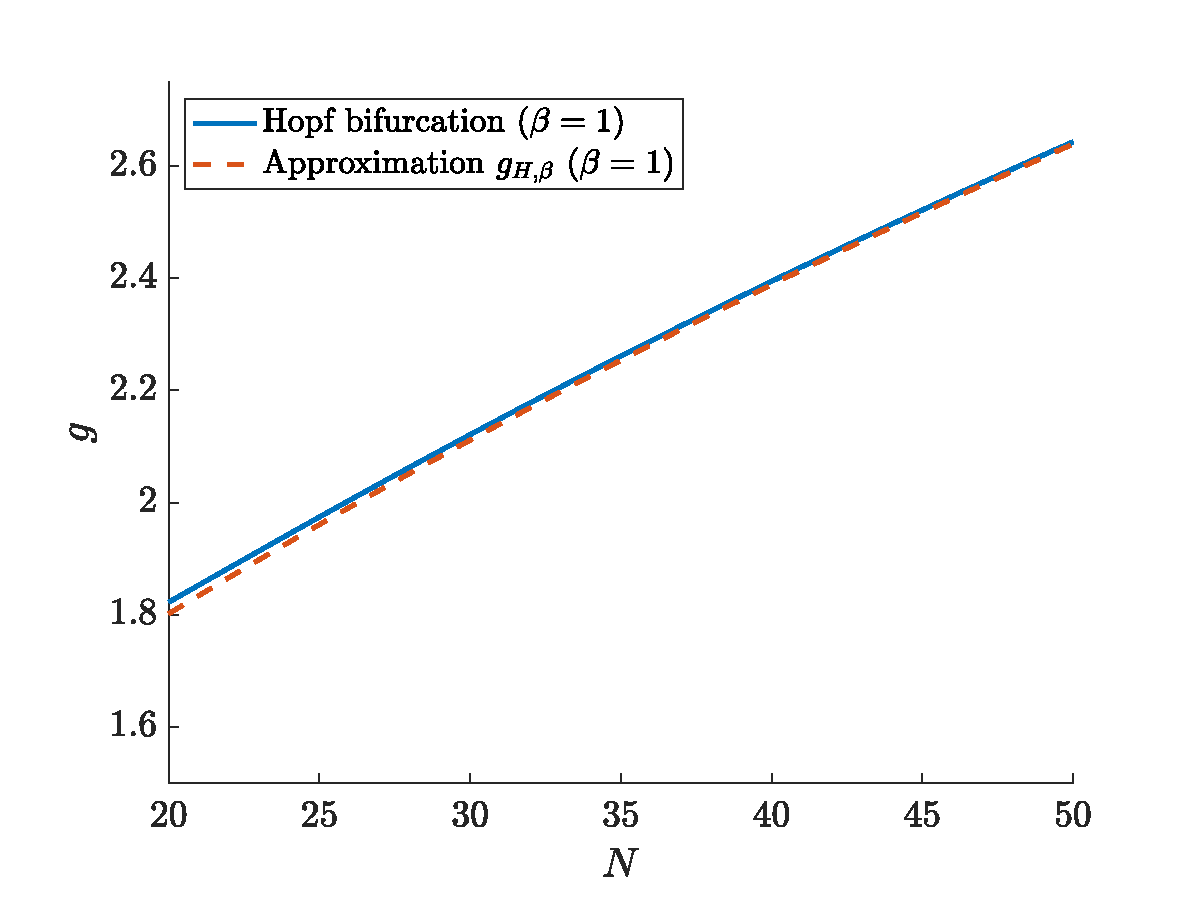
\includegraphics[width=8cm]{images/Hopfapproxbeta1.eps}
    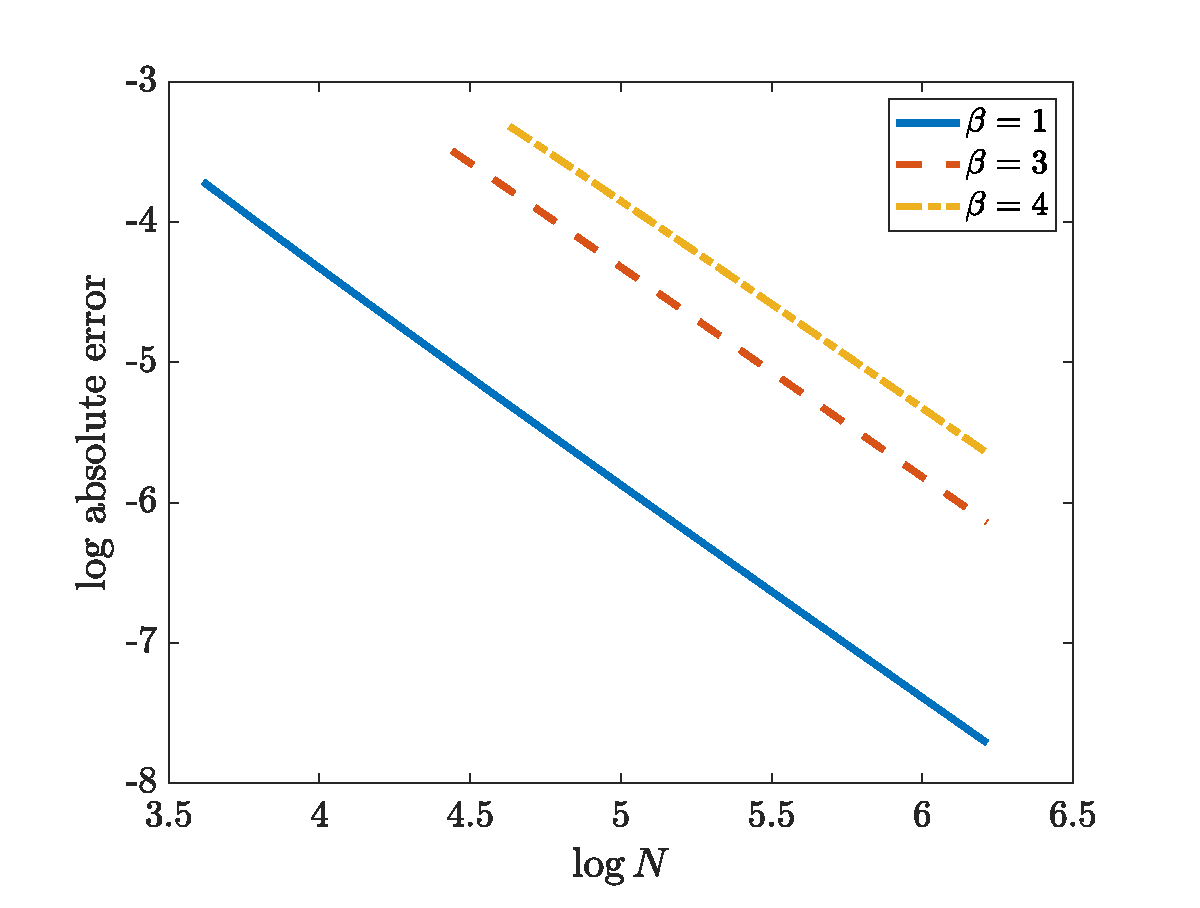
\includegraphics[width=8cm]{images/Hopfapproxerror.eps}
    \end{tabular}
    \caption{Left panel plots compares approximation \cref{eq:ghopfformula} to computed location of Hopf bifurcation for $I_1/I_2$ branch with $\beta = 1$. Right panel plots log of absolute error of approximation \cref{eq:ghopfformula} vs $\log N$ for $\beta = 1$, 3, and 4. Slope of line is approximately -1.5 for all three $\beta$. $\alpha = 4$, $\mu_{EE}= 0.7$. }
    \label{fig:Hopferror}
\end{figure}

\begin{figure}
    \centering
    \begin{tabular}{cc}
    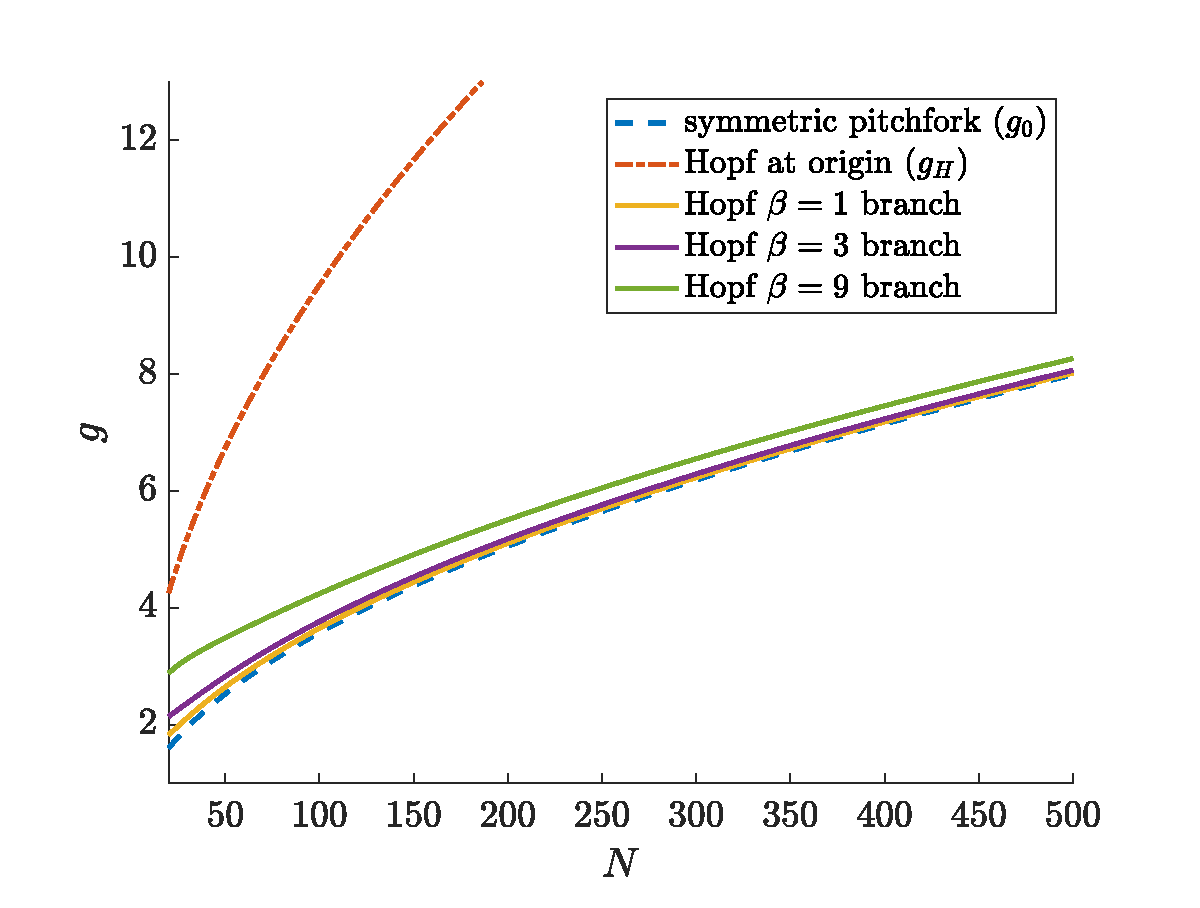
\includegraphics[width=8cm]{images/HopfNvsg.eps}
    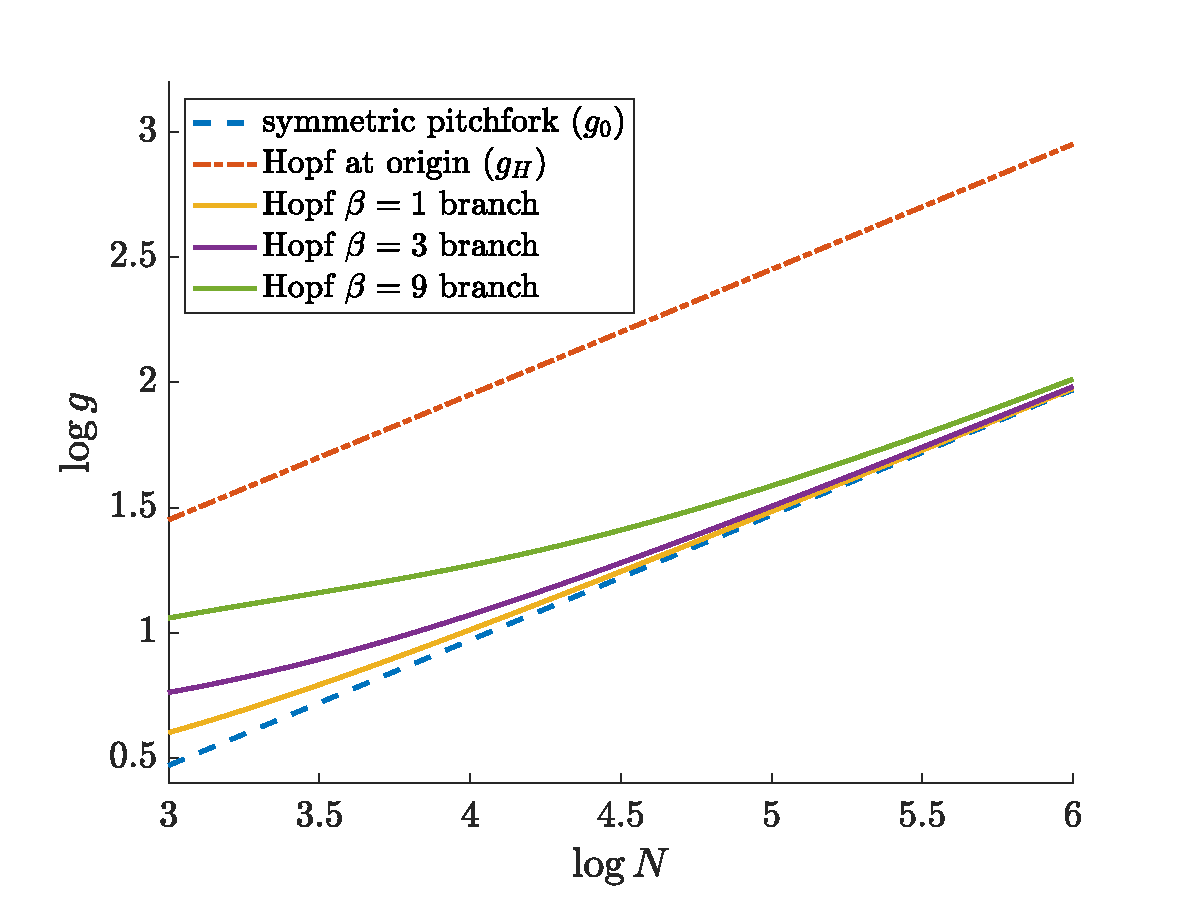
\includegraphics[width=8cm]{images/HopflogNvslogg.eps}
    \end{tabular}
    \caption{Left panel shows location in $(N, g)$ space of symmetric pitchfork bifurcation at $g_0$ (dashed line), Hopf bifurcation at origin at $g_H$ (dash-dotted line), and Hopf bifurcations on $I_1/I_2$ branches for select $\beta$ (solid lines, arranged from bottom to top in increasing $\beta$). Right panel is same data on a log-log plot.}
    \label{fig:Hopfplots}
\end{figure}
% At the Hopf bifurcation, the imaginary part of eigenvalue scales as $\sqrt{N}$, which is the frequency of oscillation of the limit cycle.

\subsection{Periodic solutions}

Periodic orbits arise from each Hopf bifurcation as $g$ increases through the bifurcation point. The periodic orbits associated with each $I_1/I_2$ branch have the same symmetry as that branch, i.e. all excitatory cells are synchronized, and the inhibitory cells are divided into two clusters of size $n_{I_1}$ and $n_{I_2}$. For the periodic orbit arising from the Hopf bifurcation at the origin at $g = g_H$, there is single excitatory cluster and a single inhibitory cluster (\cref{fig:limitcycleorigin}). 

\begin{figure}
    \centering
    \begin{tabular}{cc}
    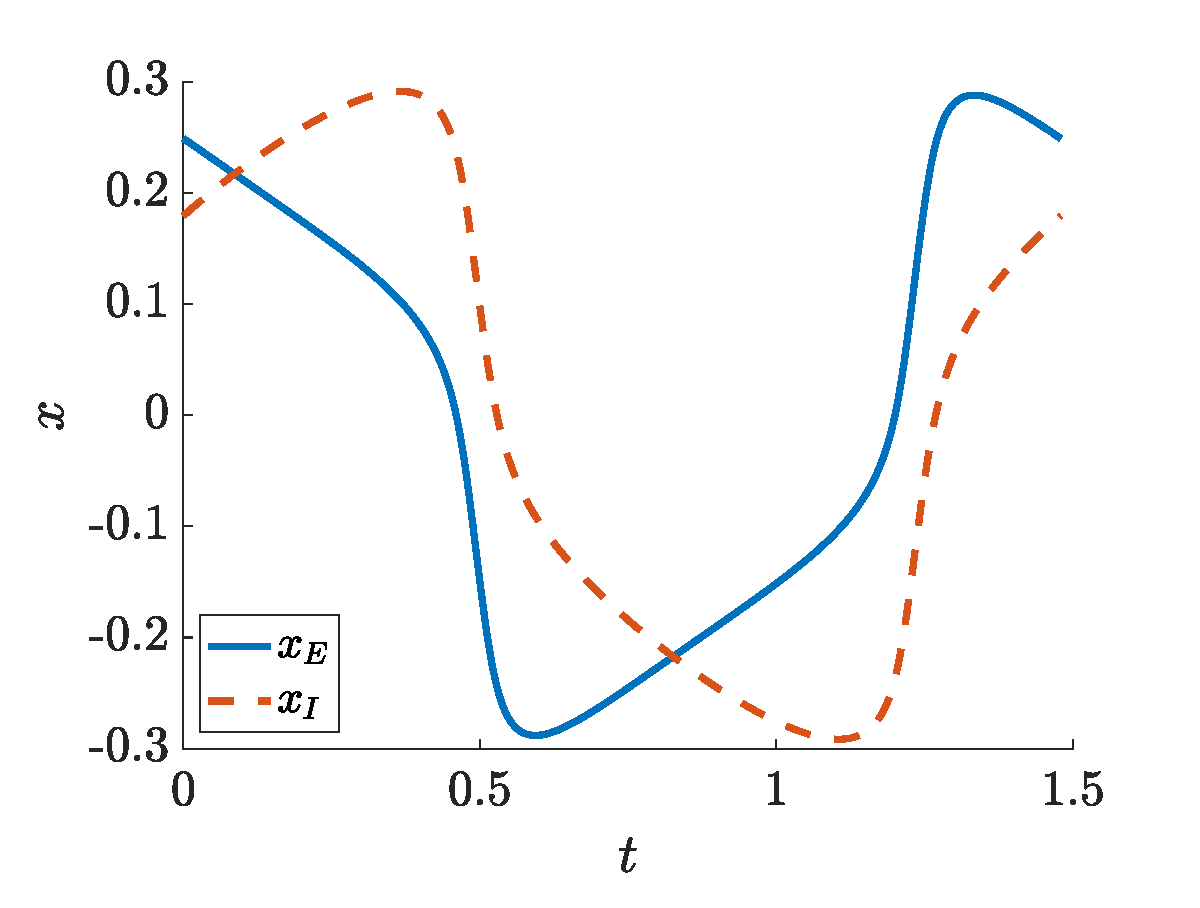
\includegraphics[width=8cm]{images/limitcycle1.eps}
    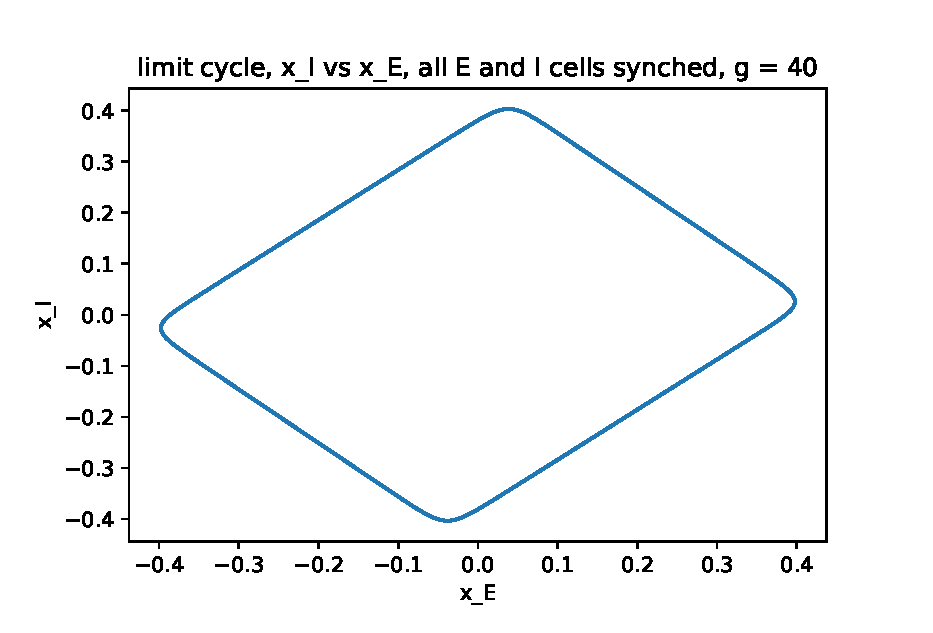
\includegraphics[width=8cm]{images/limitcycle2.eps}
    \end{tabular}
    \caption{Limit cycle arising from Hopf bifurcation at origin. Single excitatory cluster with activity $x_E(t)$, single inhibitory cluster with activity $x_I(t)$. $g = 15$, $\alpha = 4$, $\mu_{EE}= 0.7$. Period of limit cycle is 1.62.} 
    \label{fig:limitcycleorigin}
\end{figure}

\begin{figure}
    \centering
    \begin{tabular}{cc}
    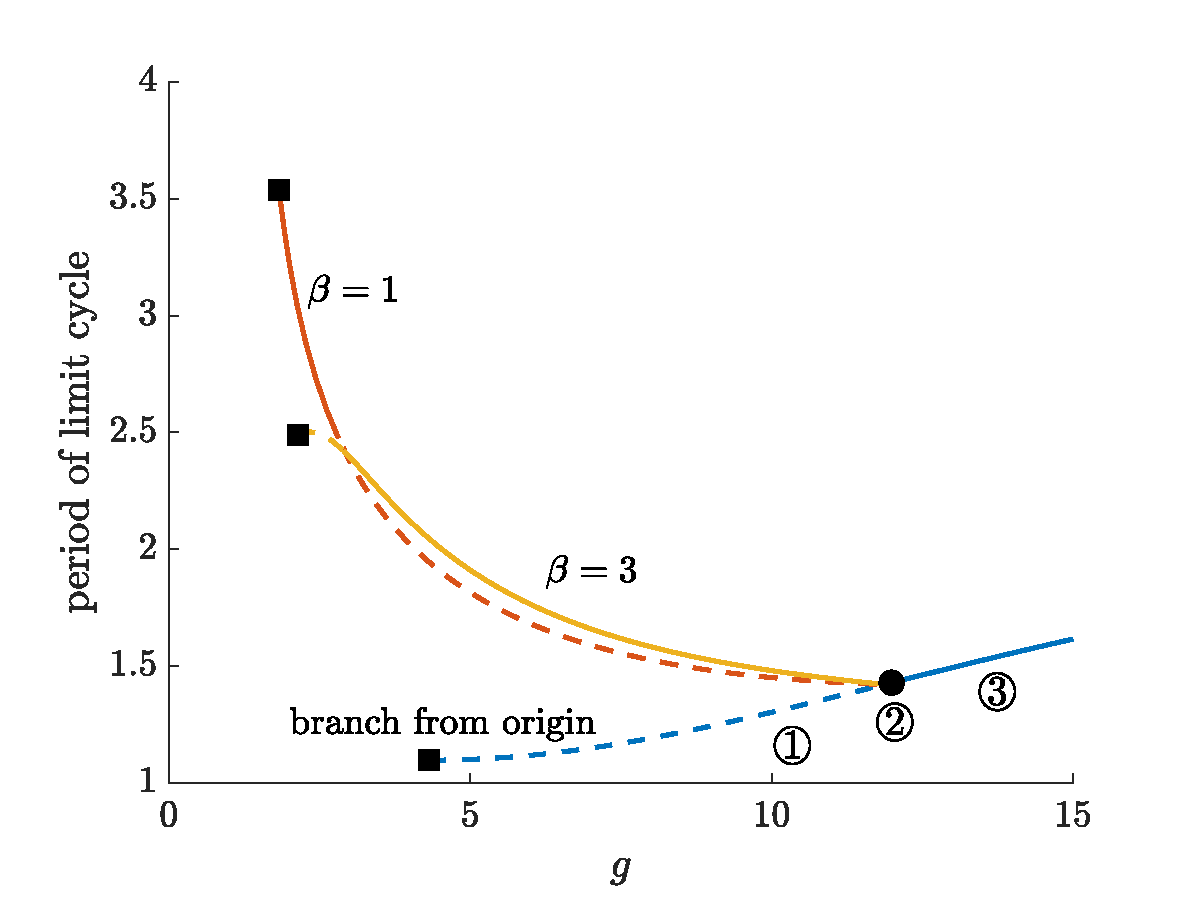
\includegraphics[width=8cm]{images/periodvsg}
    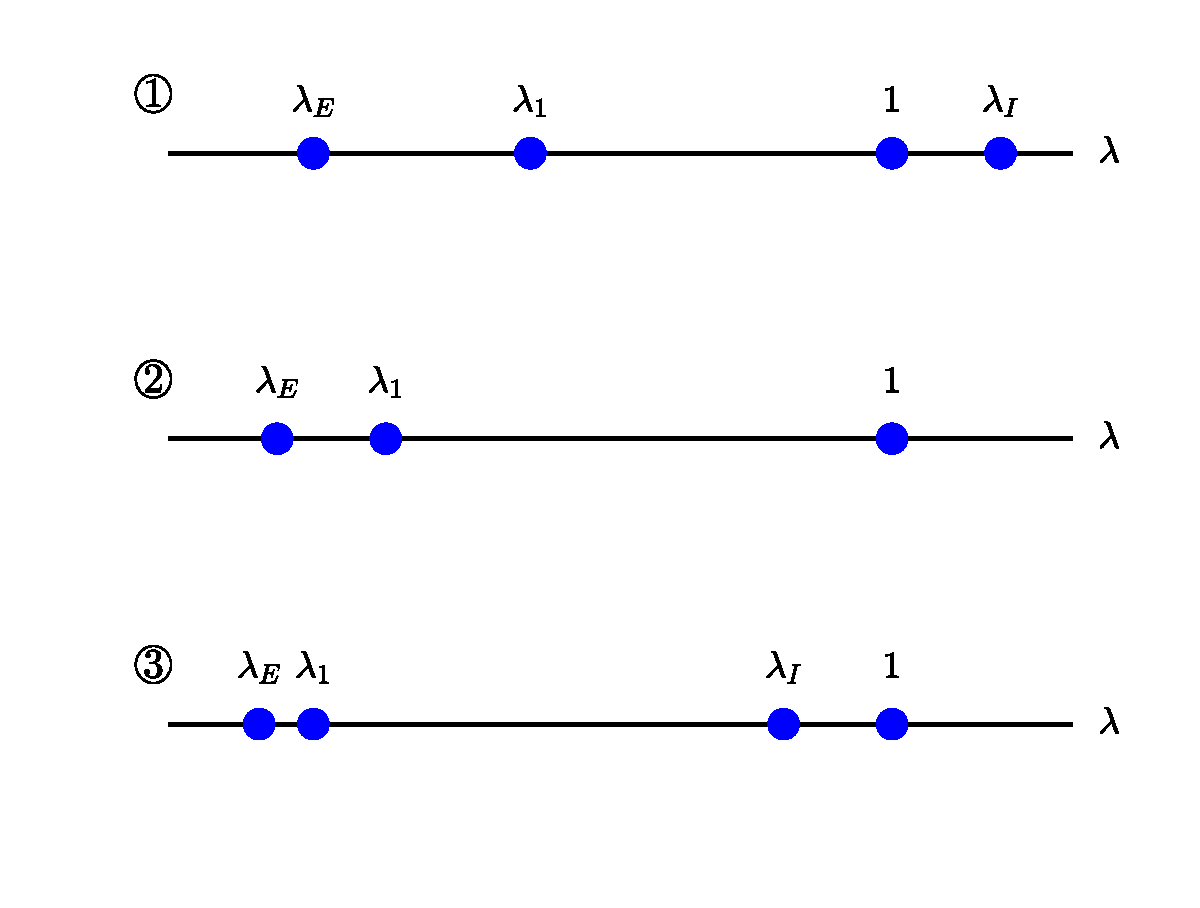
\includegraphics[width=8cm]{images/floquet1.eps}
    \end{tabular}
    \caption{Left panel shows period of limit cycle versus $g$ for periodic solutions arising from Hopf bifurcations. Stable limit cycles indicated with solid lines. Symmetric pitchfork of limit cycles is indicated with filled circle. Hopf bifurcations indicated with filled squares, which correspond to Hopf bifurcation points in \cref{fig:noclusterBD1}. Corresponding Floquet eigenvalue pattern along the branch from origin is shown in right panel.
    $N = 20$,  $\alpha = 4$, $\mu_{EE} = 0.7$.}
    \label{fig:periodvsg}
\end{figure}

A plot of the period of these limit cycles with increasing $g$ is shown in \cref{fig:periodvsg} (see also \cite{Barreiro2017}*{Figure 2}). There is a critical value $g = g_c$ where all the limit cycle branches meet. After that point, there is a single limit cycle with a single excitatory cluster and a single inhibitory cluster. This is a symmetric pitchfork bifurcation of limit cycles, which we can see by examining the Floquet multipliers of the linearization about the limit cycle branch from the origin (right panel of \cref{fig:periodvsg}). These Floquet multipliers are computed using AUTO and are all real. In addition to the single Floquet multiplier at 1 which is always present, there is a Floquet multiplier $\lambda_E$ with multiplicity $n_E - 1$, a Floquet multiplier $\lambda_I$ with multiplicity $n_I - 1$, and Floquet multiplier $\lambda_1$ with multiplicity 1. At $g = g_0$, the $n_I - 1$ Floquet multipliers $\lambda_I$ pass through 1. This is analogous to the pitchfork bifurcation of the fixed point $\xvec = 0$ at $g = g_0$, where the eigenvalue $\lambda_I$ with multiplicity $n_I - 1$ passes through the origin.

\subsection{Behavior of the $I_1/I_2$ branch for large $g$} \label{sec:stab_largeg}
We have characterized the three-cluster fixed point solutions near their origin at the symmetric pitchfork bifurcation point $g=g_0$; next, we describe how they behave for large $g$. We summarize the main points here; detailed calculations can be found in an Appendix.

Defining $y_E = \tanh(gx_E)$, etc., the equations defining a fixed point are:

 \begin{align*}
        x_E &= \frac{\mu_E}{\sqrt{N}} \left[ (n_E - 1)y_E - \alpha n_{I_1} y_{I_1} - \alpha n_{I_2} y_{I_2} \right] \\
        x_{I_1} &= \frac{\mu_E}{\sqrt{N}} \left[ n_E y_E - \alpha (n_{I_1}-1) y_{I_1} - \alpha n_{I_2} y_{I_2} \right] \\
        x_{I_2} &= \frac{\mu_E}{\sqrt{N}} \left[ n_E y_E - \alpha n_{I_1} y_{I_1} - \alpha (n_{I_2}-1) y_{I_2} \right] 
    \end{align*}
or
\begin{align}
 \begin{bmatrix} x_E\\x_{I_1}\\x_{I_2}\end{bmatrix} 
 &= \frac{\mu_E}{\sqrt{N}} 
 \begin{bmatrix} (n_E - 1) & -\alpha n_{I_1} & - \alpha n_{I_2}  \\
 n_E  & -\alpha (n_{I_1}-1) & - \alpha n_{I_2}  \\
 n_E  & -\alpha n_{I_1} & - \alpha (n_{I_2}-1)  
 \end{bmatrix}
 \begin{bmatrix} y_E\\y_{I_1}\\y_{I_2}\end{bmatrix} 
 \label{eq:3cluster_solution}
 \end{align}

Using the identity $\sech^2(y) = 1-\tanh^2(y)$, the Jacobian will be
 \begin{align}
 J &= -I + 
 \frac{g\mu_E}{\sqrt{N}} 
 \begin{bmatrix} (n_E - 1) & -\alpha n_{I_1} & - \alpha n_{I_2}  \\
 n_E  & -\alpha (n_{I_1}-1) & - \alpha n_{I_2}  \\
 n_E  & -\alpha n_{I_1} & - \alpha (n_{I_2}-1)  
 \end{bmatrix}
 \begin{bmatrix} 1-y_E^2 & 0 & 0 \\0 &  1-y_{I_1}^2 & 0\\0 & 0 &1-y_{I_2}^2\end{bmatrix} 
 \label{eq:3cluster_Jac}
 \end{align}
 Note that the diagonal matrix on the right scales each column of the non-identity portion of the Jacobian. When $y_{E/I_1/I_2}=\pm 1$, its corresponding column will be zeroed out.  
 Thus when there is a solution for which all three $y_E, y_{I_1}, y_{I_2} = \pm 1$ (rather than 0), then $J=-I$ and the solution will be stable for large $g$.

Our task is facilitated by the following observations about the behavior of the $\tanh$ function; along branches for which $x_E \rightarrow \hat{x} \not= 0$, then
\[ \tanh(gx_E) \rightarrow \left\{ \begin{matrix}
    1 & \hat{x} > 0\\
    -1 & \hat{x} < 0
\end{matrix} \right.
\] 
When this is the case Eqn. \eqref{eq:3cluster_solution} becomes linear.
If $x_E \rightarrow 0$, the limiting behavior may be more complicated; if $x_E \approx \frac{\hat{x}}{g}$, then $\tanh(gx_E) \rightarrow \tanh(\hat{x}) := y_E \not= 0$.  However, we will show it is possible to solve for the limiting coordinates and thus to characterize the stability. It turns out to be most convenient to characterize solutions by the number of coordinates that have saturating non-linearities: we itemize them as $\textbf{S0}, \textbf{S1}, \cdots$ below.

\begin{enumerate}
    \item[\textbf{S3}] If $(y_E,y_{I_1},y_{I_2}) = \pm 1$, then the non-identity matrix in Eqn. \eqref{eq:3cluster_Jac} is 0 and the solution will be stable. Unfortunately, this cannot happen; there is no solution for which \textit{all} nonlinearities saturate.
    \item[\textbf{S0}] Similarly, there is no solution for which \textit{no} nonlinearity saturates; i.e. $\tanh(g x_E) \rightarrow y_E \not= \pm 1$.
    \item[\textbf{S2}] However, for $n_{I_1} = n_{I_2}$ there is a solution for which $(y_E,y_{I_1},y_{I_2}) = (0,1,-1)$; this solution is unstable. 
    \item[\textbf{S1}] For $n_{I_1}\not=n_{I_2}$, there are solutions for which one nonlinearity saturates while the other two do not.
\end{enumerate}

% Note that the first set of equations can be written as 
% 
% \begin{align*}
% \begin{bmatrix} x_E\\x_{I_1}\\x_{I_2}\end{bmatrix} 
% &= \frac{\mu_E}{\sqrt{N}} 
% \begin{bmatrix} -y_E + C  \\
% \alpha y_{I_1} + C  \\
% \alpha y_{I_2} + C  
% \end{bmatrix}
% \end{align*}
% where $C = \frac{\mu_E}{\sqrt{N}}\left(n_E y_E -\alpha n_{I_1} %y_{I_1} - \alpha n_{I_2} y_{I_2} \right)$.


\section{Excitatory clusters, weight parameters balanced}

We now allow the excitatory cells to be grouped into $n_C$ clusters of size $p$, where $p = \lfloor N f/n_C \rfloor$. In addition, we will take $n_C \geq \alpha$ (e.g. $n_C > 4$ for the standard value of $\alpha = 4$). Since we are interested in the behavior of the system for large $N$ and for a large number of clusters (e.g. $N_c$ scales with $\sqrt{N}$), this is not a significant restriction. Cells will be connected within, but not between, clusters. The matrix $H$ is now
\[
H = \frac{1}{\sqrt{N}}
\left[ 
\begin{blockarray}{ccccc}
\begin{block}{cccc|c}
\mu_{EE}\Kvec_{p} & 0 & \hdots & 0 & \BAmulticolumn{4}{c}{\multirow{4}{*}{$\mu_{EI}\Onevec_{n_E \times n_I}$}}\\
0 & \mu_{EE} \Kvec_{p} & \hdots & 0 &&&&\\
\vdots & \vdots & \ddots & 0 &&&&\\
0 & 0 & \hdots & \mu_{EE} \Kvec_{p} &&&&\\
\end{block} 
\cline{1-8}
\begin{block}{cccc|c}
&&&&\\
\BAmulticolumn{4}{c|}{\mu_{IE}\Onevec_{n_I \times n_E}} & \mu_{II} \Kvec_{n_I}\\
\end{blockarray}
\right]
\]
which is associated with the symmetry group
\begin{align*}
\Gamma &= \underbrace{S_{p} \oplus \cdots  \oplus S_{p}}_{n_C} \oplus \, S_{n_I} && p = fN/n_C 
\end{align*}
As in the previous section, we choose the weights so that the network is balanced. To do this, the weights are related by 
\begin{align*}
\mu_{EE} &= n_C \mu && \mu_{IE} = \mu \\
\mu_{EI} &= -\alpha \mu && \mu_{II} = -\alpha
\end{align*}
The expression for $\mu_{EE}$ compensates for the fact that each excitatory cell has fewer excitatory connections. The eigenvalues of $\Hvec$ are:
\begin{itemize}
\item $\lambda_I := \alpha \mu > 0$ with multiplicity $n_I - 1$
\item $\lambda_E = -n_C \mu < 0$ with multiplicity $(p-1) \times n_C = n_E - n_C$.
\item $\lambda_C = (p-1) n_C \mu > 0$, with multiplicity $n_C - 1$.
\item A complex conjugate pair of eigenvalues $\lambda_0 \pm i \omega_0$, with 
\begin{align*}
    \lambda_0 &:= \frac{1}{2}\mu(\alpha - n_C)
      \\
    \omega_0 &:= \frac{1}{2}\mu \sqrt{ \alpha + n_C} \sqrt{ n_C(4 p - 1) - \alpha }
\end{align*}
where we used the fact that $\alpha n_I = n_E = p n_C$.
\end{itemize}
Since $\lambda_E < 0$ and $\lambda_0 \leq 0$ (since we are taking $n_C \geq \alpha$), the corresponding eigenvalues of $DF(0)$ will always be negative, and thus will not affect stability of the fixed point at 0. In particular, there will be no Hopf bifurcation at the origin. The eigenvalues which determine stability of the origin are $\lambda_I$ and $\lambda_C$. We note that for $p > 1$, i.e. we have more than one excitatory cluster, $\lambda_I < \lambda_C$.

As the bifurcation parameter $g$ increases from 0, the eigenvalue of $DF(0)$ corresponding to $\lambda_C$ crosses the imaginary axis first at 
\begin{equation}
    g = g_C := \frac{\sqrt{N}}{(p-1) n_C \mu}
\end{equation}
When this occurs, the origin loses stability in a symmetric pitchfork bifurcation. As $g$ is further increased, the eigenvalue $\lambda_I$ crosses the imaginary axis at $g = g_0$, where $g_0$ is defined by \cref{eq:pitchlocation}. An important distinction from the previous section is that there is no Hopf bifurcation at the origin, since the complex conjugate pair of eigenvalues cannot cross the imaginary axis.

It follows from Equivariant Bifurcation Theorem (as in the previous section) that there is a branch of solutions emerging at the bifurcation point $g=g_C$ for any possible division of excitatory clusters into exactly two groups of clusters. All cells are synchronized within each excitatory cluster. Each such branch may be characterized by the number $\beta_C = n_{C_1}/n_{C_2}$, which gives the ratio of the sizes of the two groups of excitatory clusters. Without loss of generality, we may take $n_{C_1} \geq n_{C_2}$, so that $\beta_C \geq 1$. For each $C_1/C_2$ branch, the inhibitory cells start out synchronized.

\subsection{Solutions on $C_1/C_2$ branch}

As in the previous section, the simplest case occurs when $n_C$ is even and $\beta_C = 1$, in which case $n_{C_1}=n_{C_2}$. On this branch, $x_{E_2} = -x_{E_1}$, i.e. there are two equally sized groups of excitatory clusters with equal and opposite activity, and all the inhibitory cells have synchronized activity $x_I = 0$. The excitatory cluster activity is given by solving 
\[
-x_E + \frac{(p-1)n_C \mu}{\sqrt{N}} \tanh(g x_E) = 0, 
\]
which simplifies to $\tanh(g x_E) = g_C x_E$. As in the previous section, $x_I$ is given, to leading order, by
\begin{align}\label{eq:xEapprox}
x_E &= \sqrt{ \frac{3(g - g_C) }{g^3}} && g \geq g_C.
\end{align}
for $g$ close to $g_C$. 

For $\beta_C > 1$, we find the solution along each $C_1/C_2$ branch by reducing \cref{eqn:sys_Basic} to the 3-dimensional system
\begin{equation}\label{eq:cluster3system}
 \begin{aligned}
 \begin{bmatrix} x_{E_1} \\ x_{E_2} \\ x_{I} \end{bmatrix} 
 &= \frac{\mu}{\sqrt{N}} 
 \begin{bmatrix} 
    (p-1)n_C & 0 & -p n_C  \\
    0  & (p-1)n_C & -p n_C \\
    p n_C \frac{\beta_C}{\beta_C+1} &
    p n_C \frac{1}{\beta_C+1} &
    -(p n_C - \alpha)
 \end{bmatrix}
 \begin{bmatrix} \tanh(g x_{E_1}) \\\tanh ( g x_{E_2} ) \\\tanh(g x_{I})\end{bmatrix},
 \end{aligned}
 \end{equation}
 where we used $\alpha n_I = n_E = p n_C$. The variables $x_{E_1}$ and $x_{E_2}$ are the activities of the two groups of excitatory clusters, and $x_I$ is the activity of the inhibitory cells (which are all synchronized). As $N \rightarrow \infty$, numerical continuation with AUTO suggests that \cref{eq:cluster3system} has a solution
\begin{equation}\label{eq:I1I2asymp}
    x_{E_2} = -\beta_C x_{E_1} + \mathcal{O}\left( \frac{1}{N^2} \right), \quad 
    x_{E_1} = \mathcal{O}\left( \frac{1}{N} \right), \quad
    x_I = \mathcal{O}\left( \frac{1}{N^2} \right)
\end{equation}
Following the same procedure as in the previous section, we obtain the formula for $x_{E_1}$
 \begin{align}\label{eq:XE1}
 x_{E_1} &= \sqrt{ \frac{ 3(g - g_C) }{ (1 - \beta + \beta^2 )g^3}} + \mathcal{O}\left( \frac{1}{N^2}\right)&& g \geq g_C,
\end{align}
for $g$ close to $g_C$, which reduces to \cref{eq:xEapprox} when $\beta = 1$.

\begin{figure}
    \centering
    \begin{tabular}{cc}
    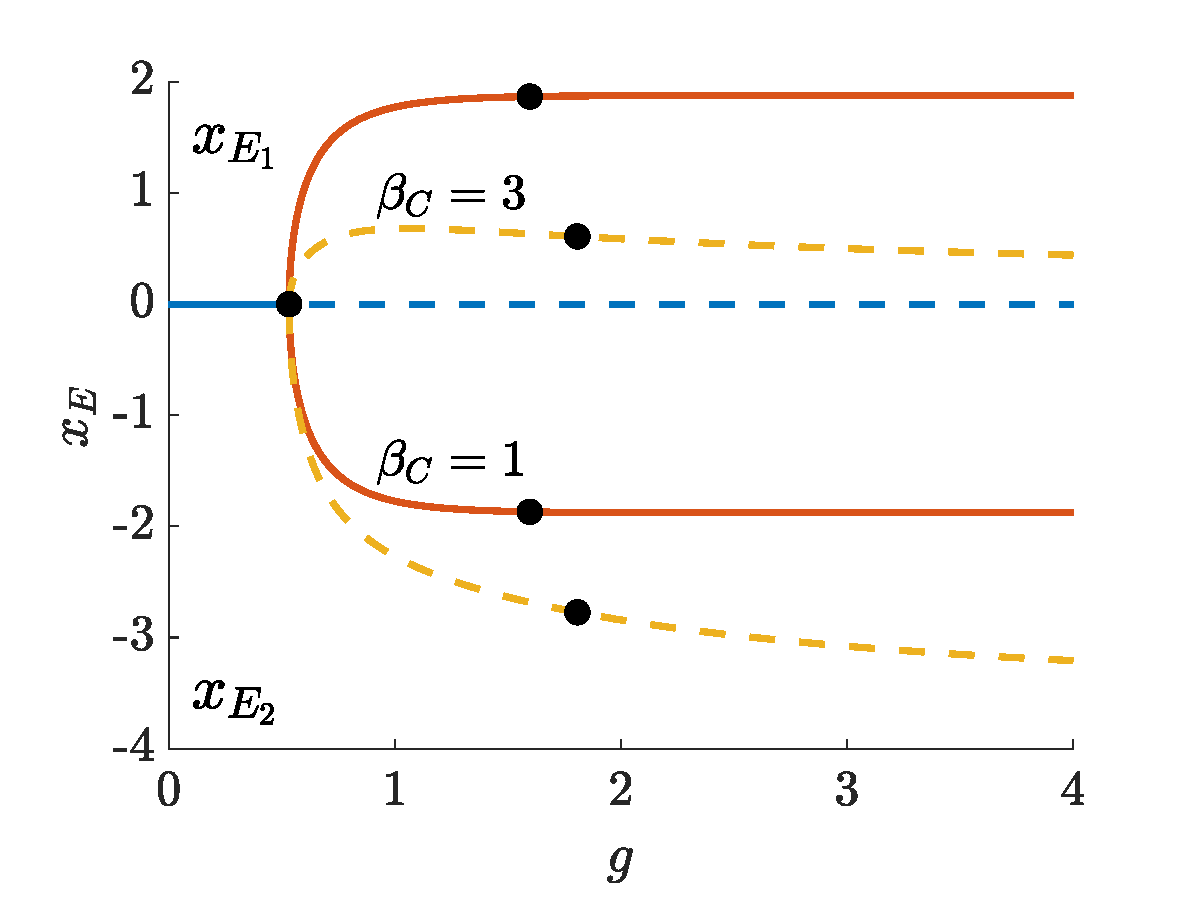
\includegraphics[width=8cm]{images/bdclusters20c4E.eps} &
    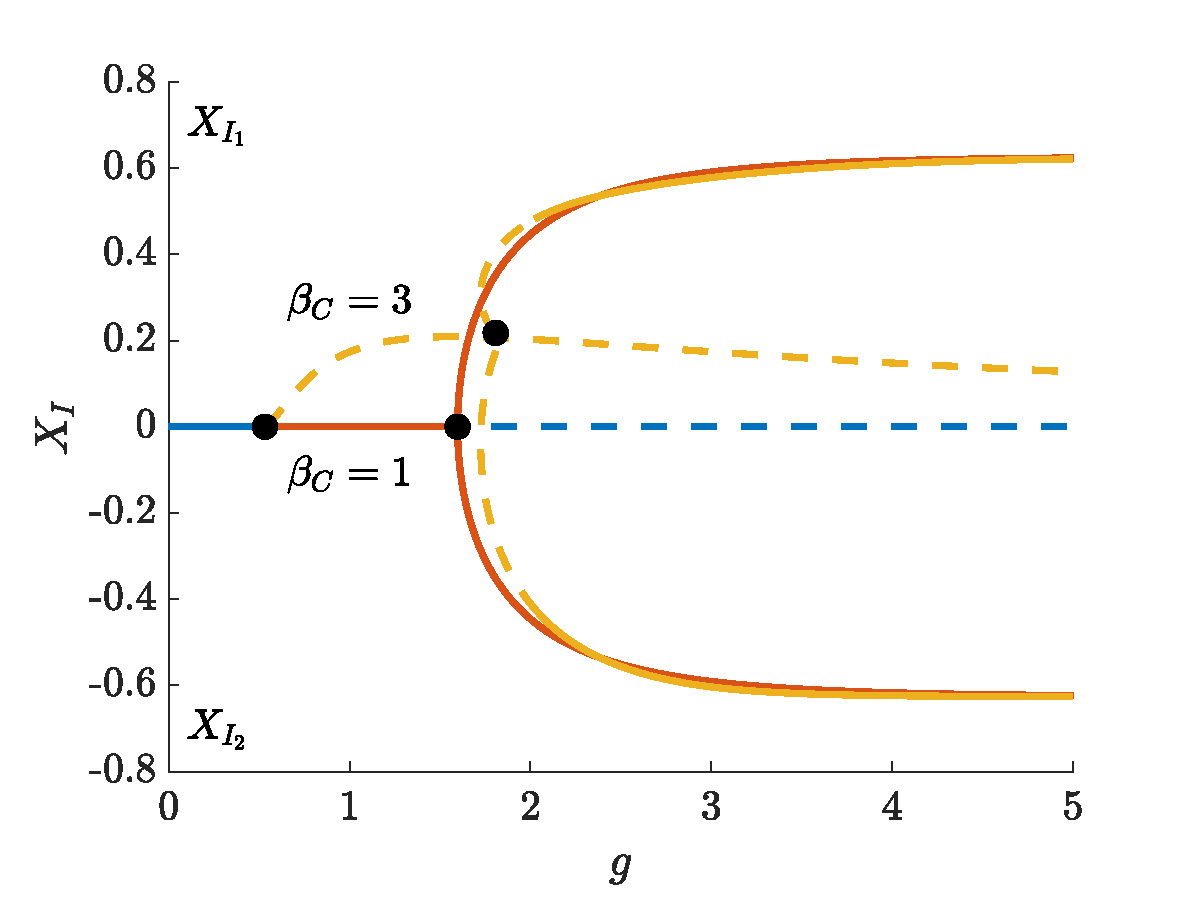
\includegraphics[width=8cm]{images/bdclusters20c4I.eps} \\
    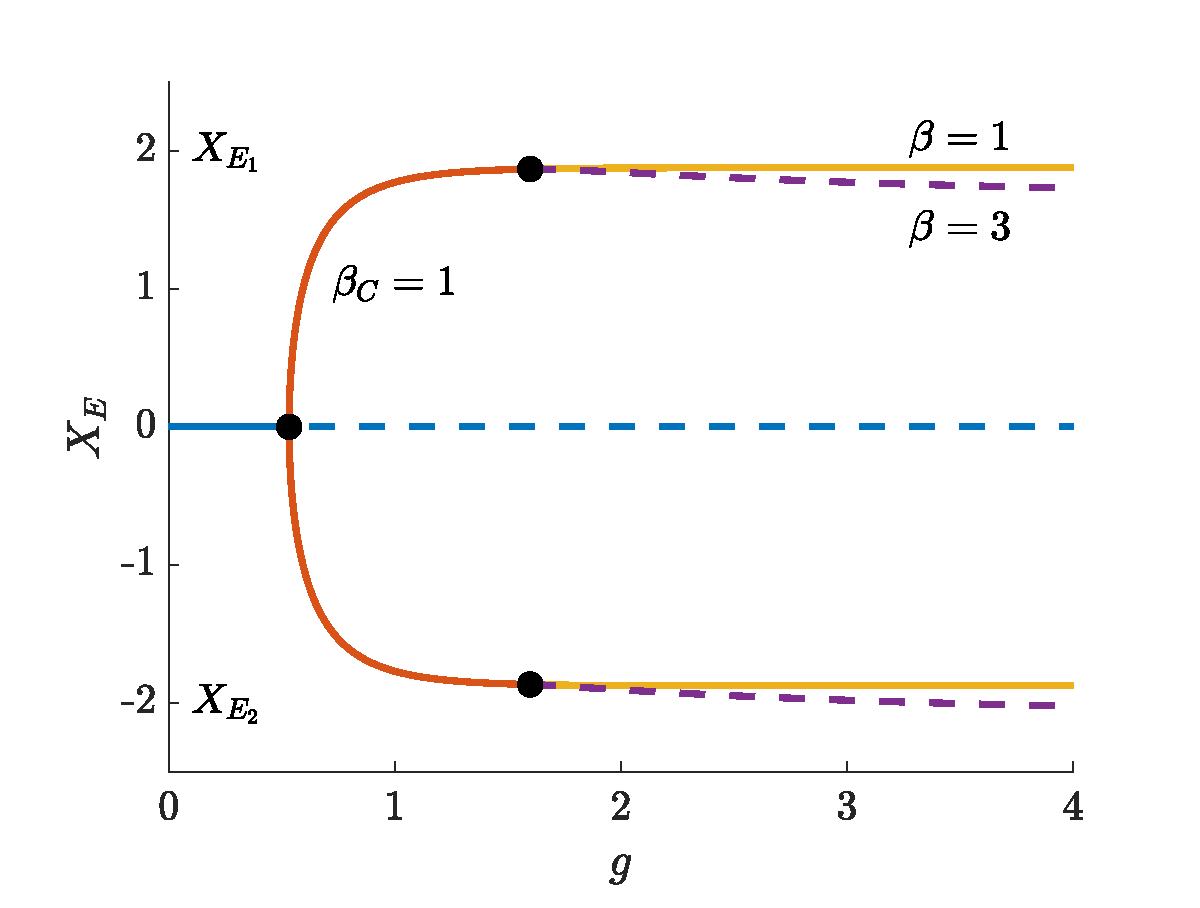
\includegraphics[width=8cm]{images/bdclusters20c4Ebetac1.eps} &
    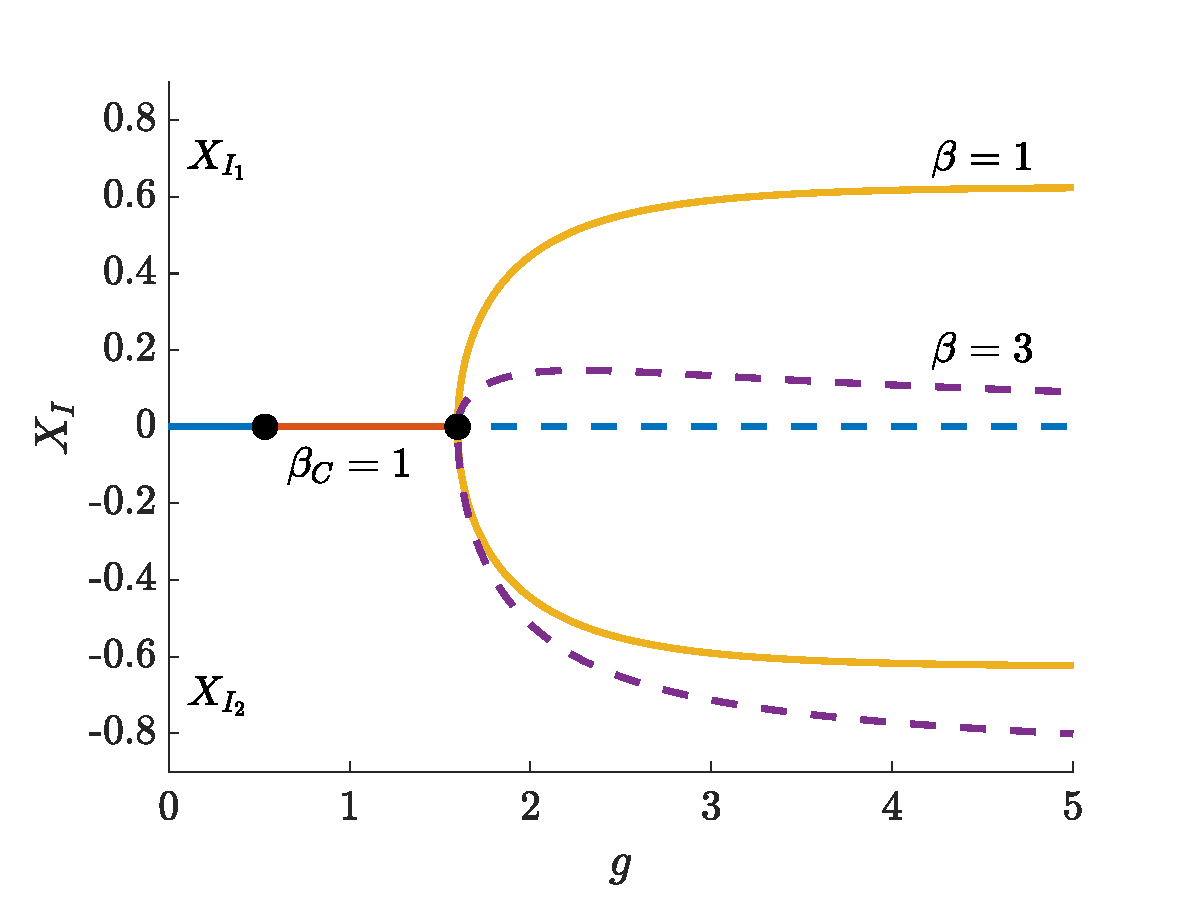
\includegraphics[width=8cm]{images/bdclusters20c4Ibetac1.eps}
    \end{tabular}
    \caption{Top panel shows bifurcation diagram showing $C_1/C_2$ branches of equilibria of \cref{eqn:sys_Basic} with excitatory clustering for all valid values of $\beta_C$, i.e. $\beta_C =1$ and $\beta_C=3$. Symmetric pitchfork bifurcations at $g = g_C$ and along the $C_1/C_2$ branches indicated wit filled circle. After symmetric pitchfork bifurcation on $C_1/C_2$ branch, only branch shown is the one with $\beta=\beta_C$ to avoid clutter. Bottom panel shows $I_1/I_2$ branches off of the $\beta_C = 1$ branch. $N = 20$, $n_C = 4$, $p = 4$, $n_I = 4$, $\alpha = 4$, $\mu_{EE} = 0.7$.}
    \label{fig:clusterBD1}
\end{figure}

\subsection{Stability and bifurcations along $C_1/C_2$ branch}

Choose any $\beta_C \geq 1$, so that $n_{E_1} = \frac{\beta_C}{\beta_C+1}n_C$ and $n_{E_2} = \frac{1}{\beta_C+1}n_C$. Let $\xvec = (x_{E_1}, x_{E_2}, x_{I})$ be a solution to \cref{eq:cluster3system}. We look at the linearization $D\tilde{F}(\xvec^*)$, where $\xvec^* = (x_{E_1}, \dots, x_{E_1}, x_{E_2}, \dots, x_{E_1}, x_{I}, \dots, x_{I})^T$, where $x_{E_1}$ and $x_{E_2}$ are repeated $n_{E_1}$ and $n_{E_2}$ times, respectively, and $x_I$ is repeated $n_I$ times. Stability will depend on the eigenvalues of $\tilde{H}(\xvec^*)$. 

We follow the same procedure as with the $I_1/I_2$ branches in the previous section.  We linearize the reduced system \cref{eq:cluster3system} about the branch $(x_{E_1}, x_{E_2}, x_{I})$ to get the Jacobian
\[
J_3(\xvec) = \frac{g}{\sqrt{N}} H_3(\xvec) - I_3
\]
where 
\[
H_3(\xvec) = \mu
\begin{bmatrix} 
    (p-1)n_C \sech^2(g x_{E_1}) & 0 & -p n_C \sech^2(g x_{I}) \\
    0  & (p-1)n_C \sech^2(g x_{E_2}) & -p n_C \sech^2(g x_{I}) \\
    p n_C \frac{\beta_C}{\beta_C+1} \sech^2(g x_{E_1}) &
    p n_C \frac{1}{\beta_C+1} \sech^2(g x_{E_2}) &
    -(p n_C - \alpha) \sech^2(g x_{I})
 \end{bmatrix}
\]
and $I_3$ is the $3 \times 3$ identity matrix. As in the previous section, the three eigenvalues of $H_3(\xvec)$ are also eigenvalues of $\tilde{H}(\xvec^*)$. Following the same procedure as in the previous section, there are $(n_{C_1}-1) + (n_{C_2}-1) + (n_I - 1)$ additional eigenvalues which are grouped as follows:
\begin{align*}
(p-1) n_C \mu &\sech^2(g x_{E_1}) &&\text{multiplicity }n_{C_1} - 1\\
(p-1) n_C \mu &\sech^2(g x_{E_2})&&\text{multiplicity }n_{C_2} - 1\\
\alpha \mu &\sech^2(g x_{I})&&\text{multiplicity }n_{I} - 1
\end{align*}
These correspond to eigenvalues of $D\tilde{F}(\xvec^*)$ which are located, to leading order, at 
\begin{align*}
&\frac{g-g_0}{g} \left( 1 - \frac{3}{1-\beta_C+\beta_C^2 }\right) \\
&\frac{g-g_0}{g} \left( 1 - \frac{3 \beta_C^3}{1-\beta_C+\beta_C^2 }\right) \\
&\frac{\alpha \mu g}{\sqrt{N}} - 1
\end{align*}
for $g$ close to $g_C$. As in the previous section, the first is negative for $1 \leq \beta_C < 2$ and positive for $\beta > 2$. The second is negative for $\beta_C  > 1/2$, and the third is negative for all $\beta$ for $N$ sufficiently large. This implies that the $C_1/C_2$ branch is initially unstable for $\beta_C > 2$. 

It remains to determine the eigenvalues of $H_3(\xvec)$. Following the same procedure as in the previous section, $H_3(\xvec)$ has a single eigenvalues which is located, to leading order, at 
\begin{align*}
    -2\left( \frac{g - g_0}{g_0} \right)  && g \geq g_0
\end{align*}
for $g$ close to $g_C$. Since this eigenvalue is always negative, it will not affect stability. $H_3(\xvec)$ also has a complex conjugate pair of eigenvalues, where the real part is given by
\begin{equation*}
\lambda(g, \beta_C) = \frac{\mu}{2}\left[ (\alpha - n_C) - \beta_C g^2 n_C (p - 1) x_{E_1}^2 \right]
\end{equation*}
to leading order. Since we are taking $n_C \geq \alpha$, this is always negative, thus there cannot be any Hopf bifurcations on the $C_1/C_2$ branch since the corresponding complex conjugate pair of eigenvalues for $J_3(\xvec)$ cannot cross the imaginary axis.

As $g$ is further increased from $g_C$, there is a second symmetric pitchfork bifurcation on each $C_1/C_2$ branch in which the group of $(n_I-1)$ eigenvalues of $D\tilde{F}(\xvec^*)$ cross the origin (see \cref{fig:clusterBD1}). The behavior at this symmetric pitchfork bifurcation is the same as in the previous section. There is an $I_1/I_2$ branch of solutions for every possible division of the inhibitory cells into exactly two clusters. We can characterize these branches using the parameter $\beta = n_{I_1}/n_{I/2}$, as in the previous section.

WE MAY BE ABLE TO FIND WHERE THE SECOND PITCHFORK BIFURCATION TAKES PLACE. IT INVOLVES $x_I$, SO DOING THIS WOULD INVOLVE A HIGHER ORDER APPROXIMATION FOR THE SOLUTIONS ON THE $C_1/C_2$ BRANCH.

\subsection{Behavior for large $g$}

Let $\mathbf{I}_n$ denote the $n\times n$ identity matrix, $\mathbf{1}_{m \times n}$ the $m\times n$ matrix of ones, and $\mathbf{K}_n$ the $n\times n$ matrix with all ones off the diagonal; i.e. $\mathbf{K}_n = \mathbf{1}_{n \times 1} \left( \mathbf{1}_{n \times 1}\right)^T - \mathbf{I}_n$. 
\begin{itemize}
\item Since we only have to solve the reduced system (one variable per excitatory cluster), define the $(N_c + N_I) \times (N_c + N_I)$ block matrix \textbf{Used xtra lines in matrix to give space: arraystretch might be better?}
\[
H_1 = \frac{1}{\sqrt{N}}
\left[ \begin{array}{c|c}
\\
(p-1)\mu_{EE} \mathbf{I}_{N_c} & \mu_{EI}\mathbf{1}_{N_c \times N_I}\\
\\
\hline
\\
p \mu_{IE} \mathbf{1}_{N_I \times N_C} & \mu_{II} \mathbf{K}_{N_I} \\
\\
\end{array}
\right]
\]

This is the original matrix $H$ (divided by $\sqrt{N}$) if you treat all excitatory cells in a single cluster as one cell.
\item For each potential large-$g$ solution, define the ``sign vector'' $\mathbf{v}$ by
\[
\mathbf{v} = (\text{sign}(x_{E1}), \dots, \text{sign} (x_{EN_c}), \text{sign} (x_{I1}), \dots, \text{sign} (x_{IN_I})
\]
where the sign is $1, -1$ or 0.
\item If a large-$g$ solution exists with that sign vector, then $H_1 \mathbf{v}$ will have the same signs as the sign vector $\mathbf{v}$ and the solution will be $H_1 \mathbf{v}$. For now, this is a necessary (but not sufficient) condition for the large-$g$ solution to exist. Hopefully it is also sufficient.
\item If all we want to know is whether such a solution can exist, we can use the relationships between the coefficients to simplify the matrix. Specifically, we assume that 
\[\begin{pmatrix}
\mu_{EE} & \mu_{EI}\\
\mu_{IE} & \mu_{II}
\end{pmatrix} \rightarrow 
\begin{pmatrix}
N_c \mu & -\alpha \mu\\
\mu & -\alpha \mu
\end{pmatrix}
 \]
 where we have expressed each coefficient in terms of $\mu = \mu_{IE}$, the $E\rightarrow I$ connection weight. Then $H_1$ simplifies 
to
\[
H_2 =
\left( \begin{array}{c|c}
(p-1)N_C\mathbf{I}_{N_c} & -\alpha \mathbf{1}_{N_c \times N_I}\\
\hline
p \mathbf{1}_{N_I \times N_C} & -\alpha \mathbf{K}_{N_I} 
\end{array}
\right)
\]
up to a constant.
%\[
%H_2 = 
%\begin{pmatrix}
%\text{diag}( (p-1)N_c) & -\alpha \\
%p & \text{offdiag}(-\alpha )
%\end{pmatrix}
%\]

Then a necessary condition for the large-$g$ solution to exist is that $H_2 \mathbf{v}$ and $\mathbf{v}$ have same signs.

\item Let $n_I^+$, $n_I^-$, and $n_I^0$ be the number of inhibitory cells which are positive, negative, and 0 in the large-$g$ limit. Let $b(I)$ be the ``balance'' of these, i.e.
\[
b(I) = n_I^+ - n_I^-
\]
Let $n_E^+$, $n_E^-$, and $n_E^0$ be the same thing for the excitatory clusters, and define the ``balance'' $b(E)$ the same way.
 
\end{itemize}

\subsubsection{Nonzero solutions}
\begin{itemize}
\item For now, assume there are excitatory clusters with both positive and negative $X_E$ and inhibitory neurons with both positive and negative $X_I$. (For homogeneous populations of one or the other, should be easier.) Also assume none of them are 0.  That is, we assume
 $n_E^+, n_E^-, n_I^+, n_I^- > 0$ and $n_E^0, = n_I^0 = 0$. Then the simplified equation 
\[ \text{sign}(H_2 \textbf{v}) = \text{sign}(\textbf{v}) \]
reduces to the conditions
\begin{align*}
&(p-1) N_c - \alpha b(I) > 0 && \text{positive excitatory} \\
-&(p-1) N_c - \alpha b(I) < 0 && \text{negative excitatory} \\
&p\:b(E) - \alpha (b(I)-1) > 0 && \text{positive inhibitory} \\
&p\:b(E) - \alpha (b(I)+1) < 0 && \text{negative inhibitory} 
\end{align*}

\item The first pair of inequalities are satisfied if and only if
\[
|b(I)| < \frac{(p-1) N_c}{\alpha}
\]
which constrains how the inhibitory cells can be split up. We can simplify the RHS using
\begin{align*}
\frac{(p-1) N_c}{\alpha}
&= (p-1) N_c \frac{N_I}{N_E}
= p N_c \frac{N_I}{N_E} - N_c \frac{N_I}{N_E} = N_I - N_c \frac{N_I}{N_E}
= N_I\left( 1 - \frac{N_c}{N_E} \right) \\
&= N_I\left( 1 - \frac{1}{p} \right)
\end{align*}
so this becomes
\[
|b(I)| < N_I\left( 1 - \frac{1}{p} \right)
\]
Since $p > 1$, this means that $|b(I)| <  N_I$, i.e. we cannot have $|b(I)| = N_I$, so there cannot be a homogeneous, nonzero population of inhibitory cells.

\item The second pair of inequalities are satisfied if and only if
\[
\frac{\alpha}{p}(b(I)-1) < b(E) < \frac{\alpha}{p}(b(I)+1)
\]
Multiply this by $N_I/N_c$ and simplify
\begin{align*}
&\frac{N_I \alpha}{N_c p}(b(I)-1) < \frac{N_I}{N_c} b(E) < \frac{N_I \alpha}{N_c p}(b(I)+1) \\
&\frac{N_I \alpha}{N_E}(b(I)-1) < \frac{N_I}{N_c} b(E) < \frac{N_I \alpha}{N_E}(b(I)+1) \\
&b(I)-1 < \frac{N_I}{N_c} b(E) < b(I)+1
\end{align*}

\item If $\frac{N_I}{N_c} b(E)$ is an integer, then we can say more, since
\[
\frac{N_I}{N_c} b(E) = b(I)
\]
which means that
\[
\frac{b(E)}{N_c} = \frac{b(I)}{N_I}
\]
Since $N_c = N_E^+ + N_E^-$ and $N_I = N_I^+ + N_I^-$, we can do some algebra to get
\[
\frac{N_E^+}{N_I^+} = \frac{N_E^-}{N_I^-} =
\frac{N_c}{N_I}
\]
from which it follows that
\[
\frac{N_E^+}{N_E^-} = \frac{N_I^+}{N_I^-},
\]
i.e. the ratio of positive to negative is the same for inhibitory cells and excitatory clusters!

\item If $\frac{N_I}{N_c} b(E)$ is not an integer, the inequalities still hold, but we no longer have the same ratio.

\end{itemize}

\subsubsection{Solutions with some zeros}

\textbf{Conjecture:} These may never happen unless the cell is 0 for all $g$.

\begin{itemize}
\item If $N_E^0 \neq 0$, i.e. there is at least one excitatory cluster which is 0 in the large $g$ limit, then we have the additional equation $0(p-1)N_c - \alpha b(I) = 0$, from which it follows that $b(I) = 0$. The inequality for $b(E)$ then becomes
\[
-\frac{\alpha}{p} < b(E) < \frac{\alpha}{p}
\]
Since $\alpha = N_E/N_I = N_c p/N_I$, this becomes
\[
-\frac{N_c}{N_I} < b(E) < \frac{N_c}{N_I}
\]
This means that if $N_c \leq N_I$, we must have $b(E) = 0$ as well. There are more possibilities if $N_c > N_I$.

\item If $N_I^0 \neq 0$, i.e. there is at least one inhibitory cluster which is 0 in the large $g$ limit, then we have the additional equation 
\[
p b(E) - \alpha b(I) = 0
\]
which implies
\[
b(E) = \frac{\alpha}{p} b(I) = \frac{N_c}{N_i} b(I)
\]

\end{itemize}

\subsubsection{Solutions with $\tanh(gx) \rightarrow r$, $0 < \vert r \vert < 1$}

A final possibility is that there are degrees of freedom for which $x_k \rightarrow 0$, but in such as way that $g x_k \rightarrow c$ for some real constant $c$. Then $\tanh(gx) \rightarrow r$, $0 < \vert r \vert < 1$. Deriving such solutions becomes considerably more complicated, as we have not only a linear matrix equation, but nonlinear consistency conditions relating $x_k$ and $\tanh(g x_k)$ \textbf{Actually LHS is zero for large g: still more complicated than $\pm$ 1}

Instead of proceeding along these lines, we will show that all such solutions are unstable.

\subsection{Excitatory clusters with weight parameters unchanged}

We can also choose the weights as in the previous section, i.e. $\mu_{EI} = -\alpha \mu_{EE}$, $\mu_{II} = -\alpha \mu_{EE}$, and $\mu_{IE} = \mu_{EE}$. In this case, the two eigenvalues of $H$ with positive real part are $\lambda_I = \alpha \mu_{EE}$ and $\lambda_C = (p-1)\mu_{EE}$. If $\lambda_C > \lambda_I$, which occurs when $n_C < \frac{f N}{\alpha+1}$, the behavior is qualitatively the same as for the case balanced weight parameters discussed above. If  $\lambda_C < \lambda_I$, which occurs when $n_C > \frac{f N}{\alpha+1}$, the order of the two symmetric pitchfork bifurcations is reversed. As $g$ is increased, the inhibitory cells bifurcate from the origin first, followed by the excitatory clusters.

\section{Inhibitory clusters}

We can also allow the inhibitory cells to be clustered, while the excitatory cells remain unclustered. Briefly, suppose the inhibitory cells are grouped into $n_{C_I}$ inhibitory clusters of size $p_i$. For the choice of weights $\mu_{EI} = -\alpha \mu_{EE}$, $\mu_{II} = -\alpha \mu_{EE}$, and $\mu_{IE} = \mu_{EE}$, the eigenvalues of $\Hvec$ can be obtained by reversing the role of the excitatory and inhibitory cells in the previous section:
\begin{itemize}
\item $\lambda_I := \alpha \mu_{EE} > 0$ with multiplicity $(p_I-1) \times n_{C_I} = n_I - n_{C_I}$.
\item $\lambda_E = -\mu_{EE} < 0$ with multiplicity $n_E - 1$
\item $\lambda_{C_I} = -(p_I-1)\alpha \mu_{EE} < 0$, with multiplicity $n_{C_I}-1$.
\item A complex conjugate pair of eigenvalues $\lambda_0 \pm i \omega_0$, with 
\begin{align*}
    \lambda_0 &:= \frac{1}{2}\mu_{EE} \left[ \alpha( 1 + p_I(n_{C_I}-1)) -1 \right]
      \\
    \omega_0 &:= \sqrt{a^2 \left(\left(-3 n_{C_I}^2+2 n_{C_I}+1\right) p_I^2-2 (n_{C_I}+1) p_I+1\right)-2 a
    (n_{C_I}p_I +p_I -1)+1}
\end{align*}
where we used the fact that $n_E = \alpha n_{C_I} p_I$.
\end{itemize}
The only two eigenvalues with positive real part are $\lambda_I$ and $\lambda_0 + i \omega_0$, so those are the only ones which will cause bifurcations as $g$ is varied. We note that $\lambda_0 > \lambda_I$, thus the first bifurcation which will occur at the origin as $g$ is increased from 0 is a Hopf bifurcation at 
\[
g_H = \frac{2 \sqrt{N}}{\mu_{EE} \left[ \alpha( 1 + p_I(n_{C_I}-1)) -1 \right] }
\]
We are interested in what occurs for large $N$ and large $N_{C_I}$. As an example, let $N_{C_I}$ scale with $\sqrt{N}$, so that $N_{C_I} = p_I = \sqrt{N}$. For this scaling, as $N$ increases, the Hopf bifurcation takes place at $g_H \approx \frac{2}{f \mu_{EE} \sqrt{N}}$. For large $N$, we also have $\omega_0 \approx \frac{\sqrt{3}}{2}f N \mu_{EE}$. Thus, at $g = g_H$, $DF(0)$ has a complex conjugate pair of eigenvalues with real part of 0 and imaginary part of $\sqrt{3}$. This implies that for large $N$, the frequency of the limit cycle emerging at the Hopf bifuration of the origin is asymptotically constant as $N$ increases.


We can also choose the weights so that the network is balanced, as in the previous section. In that case, the eigenvalues of $\Hvec$ are
\begin{align*}
\mu_{EE} &= \mu && \mu_{IE} = \mu \\
\mu_{EI} &= -\alpha \mu && \mu_{II} = -\alpha n_{C_I} \mu
\end{align*}
The eigenvalues of $\Hvec$ can be obtained by reversing the role of the excitatory and inhibitory cells in the previous section:
\begin{itemize}
\item $\lambda_I := \alpha n_{C_I} \mu > 0$ with multiplicity $(p_I-1) \times n_{C_I} = n_I - n_{C_I}$.
\item $\lambda_E = -\mu < 0$ with multiplicity $n_E - 1$
\item $\lambda_{C_I} = -(p_I-1) \alpha n_{C_I} \mu < 0$, with multiplicity $n_{C_I} -1$.
\item A complex conjugate pair of eigenvalues $\lambda_0 \pm i \omega_0$, with 
\begin{align*}
    \lambda_0 &:= \frac{1}{2}\mu(\alpha n_{C_I} - 1)
      \\
    \omega_0 &:= \frac{1}{2}\mu \sqrt{ \alpha n_{C_I}+1} \sqrt{\alpha n_{C_I}(4p_I - 1) - 1}
\end{align*}
\end{itemize}



Key here is that the complex pair crosses the imaginary axis first as $g$ is increased, leading to a Hopf bifurcation and a stable limit cycle. The real part of this complex pair $\lambda \pm i \omega$ is given by
\begin{align*}
\lambda &= -\frac{\mu_{II} (1-f)N}{2}\left( 1 - \frac{1}{N_{ci}} + \frac{1}{N(1-f)}\left( 1 - \frac{1}{\alpha} \right) \right) \\
&\approx -\frac{\mu_{II} (1-f)N}{2}\left( 1 - \frac{1}{N_{ci}} \right) && \text{for $N$ large } \\
&\approx -\frac{\mu_{II} (1-f)N}{2} && \text{for $N$ and $N_{ci}$ large } \\
\end{align*}
which grows with $N$. This means that the Hopf bifurcation takes place at approximately
\[
g \approx g_0 \approx -\frac{2}{(1-f)\mu_{II}\sqrt{N}} 
\]
for large $N$ and $N_c$. The frequency of oscillations of the limit cycle is given by the imaginary part of the complex pair, which is approximately
\begin{align*}
\omega &\approx -\frac{\mu_{II} (1-f)N}{2 N_{ci} } \sqrt{ 3 N_{ci}^2 - 2 N_{ci} - 1} && \text{for $N$ large } \\
&\approx -\frac{\sqrt{3} \mu_{II} (1-f)N}{2 } && \text{for $N$ and $N_{ci}$ large }
\end{align*}
which also grows with $N$. At the Hopf bifurcation, which is at $g = g_0$, after scaling by $N$ and $g$, we have
\[
\omega \rightarrow \sqrt{3} \text{ as } N, N_{ci} \rightarrow \infty
\]
which is independent of everything. This assumes the same balance of inhibitory and excitatory neurons as before, as well as $\mu_{II} = -\alpha \mu_{EE}$, etc from the initial excitatory cluster case. 

Appears that this periodic orbit is stable for all $g > g_0$. For this orbit, all inhibitory cells and all excitatory cells synced. Frequency decreases as $g$ increases, also shape of oscillations changes.

\begin{figure}[H]
\centering
\begin{tabular}{cc}
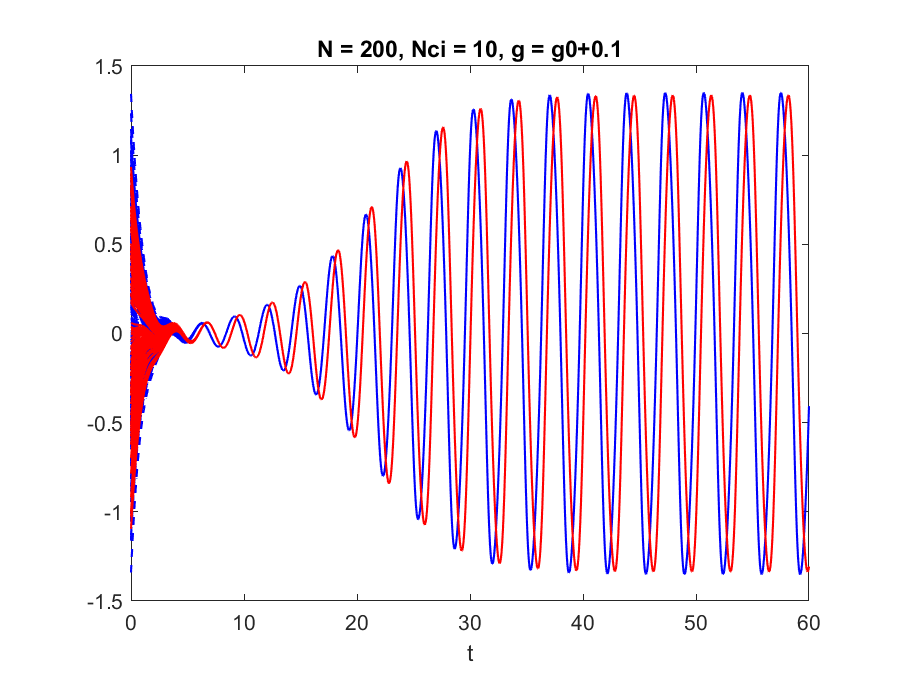
\includegraphics[width=8cm]{images/Iclustertimestep400_1.eps} &
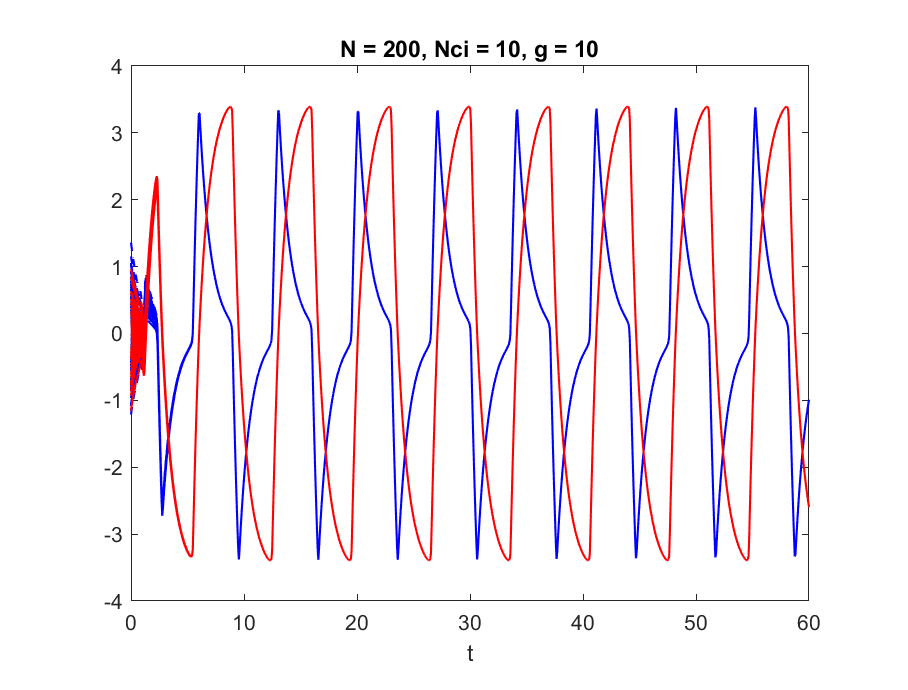
\includegraphics[width=8cm]{images/Iclustertimestep400_2.eps}
\end{tabular}
\end{figure}

\section{Appendix}
\subsubsection{Detailed calculations for \S \ref{sec:stab_largeg}}

We are seeking solutions to 
 \begin{align}
 \begin{bmatrix} x_E\\x_{I_1}\\x_{I_2}\end{bmatrix} 
 &= \frac{\mu_E}{\sqrt{N}} 
 \begin{bmatrix} (n_E - 1) & -\alpha n_{I_1} & - \alpha n_{I_2}  \\
 n_E  & -\alpha (n_{I_1}-1) & - \alpha n_{I_2}  \\
 n_E  & -\alpha n_{I_1} & - \alpha (n_{I_2}-1)  
 \end{bmatrix}
 \begin{bmatrix} y_E\\y_{I_1}\\y_{I_2}\end{bmatrix} 
 \label{eqn:matSolgLrg}
 \end{align} 
 where $y_E = \tanh(gx_E)$, etc..
 Recall that if such a solutions can be found, its stability will be governed by the Eqn. 
 
 As $g \rightarrow \infty$, both the solutions and Jacobian simplify because the nonlinearities saturate to a constant value: if $x \rightarrow \hat{x} \not= 0$, then
\[ \tanh(gx) \rightarrow \left\{ \begin{matrix*} 1 & x > 0\\
    -1 & x < 0
    \end{matrix*}
    \right.
 \] 
 We will characterize solutions based on how many coordinates (i.e. $x_E, x_{I_1}$, and $x_{I_2}$) saturate in this way.
 
 Note that if all three coordinates $y_{E/I_1/I_2}=\pm 1$, then $J=-I$ and the solution will be stable for large $g$.
 Therefore we will start there. We ask if there is a vector of $\pm 1$, $(y_E, y_{I_1}, y_{I_2})$, whose image under this equation lies in the same octant (\textbf{S3}).
 \begin{itemize}
     \item Assume WLOG that $y_{I_1}>0$ and $y_{I_2}<0$. Define the balance $b = n_{I_1}-n_{I_2}$. Then our equations for $y_{I_1},y_{I_2}$ become
     \begin{align*}
        n_E y_E - \alpha(b-1) &>0\\
        n_E y_E - \alpha(b+1) &<0
     \end{align*}
     or, using the identity $n_E = \alpha n_I$,
     \[ n_I y_E - 1 < b < n_I y_E + 1 \]
     \item If $y_E=1$ then $n_I-1 < b < n_I+1$; if $y_E=-1$ then $-n_I-1 < b < -n_I+1$. Combining these two observations, either
     \[ b < -n_I + 1 \qquad \text{or} \qquad b > n_I - 1 \]
     
     However, the possible values of $b$ are limited by $n_I$: $n_{I_1}=n_I-1 \rightarrow b = n_I-1-1  = n_I-2$,  in fact
     \[ -n_I + 2 \leq b \leq n_I -2 \]
     neither option is possible! 
     \item The final option is that $y_E = 0$. This can only hold if $b=0$ i.e. $n_{I_1}=n_{I_2}$. The Jacobian in this case is
     \[ J = -I + \frac{g\mu}{\sqrt{N}}
     \begin{bmatrix} (n_E-1) & 0 & 0\\
        n_E & 0 & 0\\
        n_E & 0 & 0 \end{bmatrix}\]
        where we use $\sech^2(g x_{I_1}) = 0$, $\sech^2(gx_E)=1$.
        This solution is unstable for $g > \frac{\sqrt{N}}{\mu (n_E-1)}$
 \end{itemize}
 THis shows that while there is no solution of the form $\textbf{S3}$, there is one solution of the form $\textbf{S2}$.
 
Next, we consider the possibility that 
 $\tanh(gx) \rightarrow y$ but $0 < y < 1$ or $-1 < y < 0$ for each coordinate. In this case 
\[ x \approx \frac{\tanh^{-1}(y)}{g} \]

However, in Eqn. \eqref{eqn:matSolgLrg} the left-hand side must go to the zero vector as $g \rightarrow \infty$; thus the vector with the limiting values of $y_E$, $y_{I_1}$ and $y_{I_2}$ must be in the nullspace of the matrix in Eqn. \eqref{eqn:matSolgLrg}. 
This matrix is full rank! So there is no solution for which $x \rightarrow 0$ but $\tanh(gx) \rightarrow a$, where $0 < |a| < 1$, for all three values $x = x_E, x_{I1}, x_{I2}$. (\textbf{S0}).

Finally we show that the remaining $I_1/I_2$ branches have solutions of the form $\textbf{S1}$.
It turns out that what can happen is that, for example, $x_{E}, x_{I_1} \rightarrow 0$ as $g \rightarrow \infty$, but that $x_{I2}$ has a nonzero limit as $g \rightarrow \infty$ (see \cref{fig:20symm1} for an example of this exact occurrence for 1:1 and 3:1 I-cell symmetry in the $N=20$ case). Then we have $\tanh(g x_E), \tanh(g x_{I1})$ approaching a limit between 0 and 1 as $g \rightarrow \infty$ and $\tanh(g x_{I2}) \rightarrow 1$ as $g \rightarrow \infty$.

What are necessary conditions for such a solution to exist? Let us solve
\[ A \begin{bmatrix} y_1\\y_2\\y_3\end{bmatrix} = A \textbf{y} = \textbf{e}_k 
\]
where $\textbf{e}_k$ is the $k$th unit vector.

Then the following must be true:
\begin{enumerate}
    \item[\textbf{C1:}] $(\textbf{y})_k > 0$
    \item[\textbf{C2:}] $|(\textbf{y})_k| > |(\textbf{y})_j|$ for any $j\not=k$. 
\end{enumerate}
We can then obtain our desired $\begin{bmatrix} y_E\\y_{I_1}\\y_{I_2}\end{bmatrix} $ by dividing $\textbf{y}$ by its maximum.

% This is a necessary but not sufficient condition. The figure below shows the solution $y_E = 0.2222$, $y_{I_1}=-0.0556$, $y_{I_2}=1$, which we can obtain by using $\textbf{e}_3$ and normalizing the vector so that its largest entry is 1.

% However, there is a second possibility, using $\textbf{e}_2$, for which $y_E = 0.75$, $y_{I_1}=1$, $y_{I_2}=-0.1875$, which does not appear to correspond to an actual solution branch.

It turns out it is easy to invert $A$, using Cramer's rule:

\begin{align*}
   A^{-1} & = \frac{1}{\alpha^2 (N-1)}\begin{bmatrix}
    -\alpha^2 (n_I-1) & \alpha^2 n_{I_1} & \alpha^2 n_{I_2}\\
    -\alpha n_E & \alpha (n_E + n_{I_2}-1) & -\alpha n_{I_2}\\
    -\alpha n_E & -\alpha n_{I_1} & \alpha (n_E + n_{I_1}-1)\\
    \end{bmatrix}
\end{align*}

Note that $\textbf{C1}$ is met for $\evec_2$ and $\evec_3$, but is never met for $\evec_1$.
However, using $n_E = \alpha n_I$ and $\alpha > 1$, we can see that
\[ \alpha (n_E + n_{I_2}-1)> \alpha^2 n_{I_1} > \vert -\alpha n_{I_1}\vert \]
and
\[ \alpha (n_E + n_{I_1}-1)> \alpha^2 n_{I_2} > \vert -\alpha n_{I_2}\vert \]
i.e. \textbf{C2} is also met for both $\evec_2$ and $\evec_3$.

Therefore we have two solutions, each of which can be seen (for example) as the positive and negative parts of the 1:3 solution curve in Fig. \#\#:
\begin{eqnarray}
\begin{bmatrix} y_E\\y_{I_1}\\y_{I_2}\end{bmatrix} & = & \begin{bmatrix} \frac{\alpha n_{I_1}}{N-n_{I_1}-1}\\
    1 \\ -\frac{n_{I_1}}{N-n_{I_1}-1}
\end{bmatrix}
\label{eq:S1_sol1}
\end{eqnarray}
and 
\begin{eqnarray}
\begin{bmatrix} y_E\\y_{I_1}\\y_{I_2}\end{bmatrix} & = & \begin{bmatrix} \frac{\alpha n_{I_2}}{N-n_{I_2}-1}\\
    -\frac{n_{I_2}}{N-n_{I_2}-1}\\1
\end{bmatrix}.
\end{eqnarray}
For each solution, the value of the ``saturated" coordinate ($x_{I_1}$ or $x_{I_2}$) in the limit $g \rightarrow \infty$ is given by multiplying 
the vector above by $A$; for Eqn. \eqref{eq:S1_sol1},
\[ x_{I_1} = \frac{\alpha \mu_{EE}}{\sqrt{N}} \frac{N-1}{N-n_{I_1}-1}\]
Then for a finite $g$, recover the other coordinates using
\[ x_E = \frac{1}{g} \tanh^{-1}\left( \frac{\alpha n_{I_1}}{N-n_{I_1}-1}\right); \qquad  x_{I_2} = \frac{1}{g} \tanh^{-1}\left( -\frac{n_{I_1}}{N-n_{I_1}-1}\right)\]

To assess stability, return to Eqn. \eqref{eqn:Jmat_3pop}: writing $J = -I + \frac{g\mu_E}{\sqrt{N}} \tilde{J}$, we find that 
\[ {\rm tr} (\tilde{J})  = (1-y_E^2)(n_E-1) - (1-y_{I_1}^2)\alpha(n_{I_1}-1) \]


\bibliographystyle{amsplain}
\bibliography{main.bib}

\end{document}
